\chapter{Modelling a Database for Dynamic Multimedia Data}
\label{chapter:system_model}
\epiquote{The science of operations, as derived from mathematics more especially, is a science of itself, and has its own abstract truth and value.}{Ada Lovelace, 1843}

We have argued in \Cref{chapter:applications} that multimedia retrieval, analysis and analytics workloads (and workloads that exhibit similiar characteristics) pose specific requirements on a database system. In this chapter, we focus on four aspects and derive a formal model to accomodate them on a systems level:

\begin{description}
    \item[Support for Complex Data Types] Multimedia workloads process features that are often real-valued, high-dimensional vectors but can be any type of mathematical object (e.g., complex numbers). A multimedia \acrshort{dbms} must support these objects as first-class citizens (see \Cref{requirement:complex_data_types}).
    \item[Support for Distance Computation] The notion of proximity between features plays a crucial role in all types of multimedia workloads, which involves the evaluation of functions. A multimedia \acrshort{dbms} must be able to execute these funcitons efficiently, using the available data structures and execution methods (see \Cref{requirement:functions}).
    \item[Dynamic Data] Data is usually subject to constant change and a multimedia \acrshort{dbms} must be able to propagate these changes to all the relevant data structures while maintaining an internal consistency model (see \Cref{requirement:big_data} and \Cref{requirement:classical_dbms}).
    \item[Quality vs. Time] Multimedia queries often trade retrieval quality against speed or vice-versa, e.g., when using a high-dimensional indexes. A multimedia \acrshort{dbms} must make these decisions explicit and allow the user to express their perference at different levels of the system (see \Cref{requirement:quality_model}).
\end{description}

To address these requirements, we propose and formalise a set of functionality, which will be specified in the next sections. First, we propose a notion of \emph{generalised, proximity based queries} as an extension to the relational model. Second, we describe a \emph{cost-model} that takes the notion of quality of results into account. And finally, we introduce the formal requirements to enable high-dimensional indexes to cope with dynamic data and derive a model for maintaining such indexes. All these contributions can be seen as extensions to the functionality provided by a traditional \acrshort{dbms}. To establish a frame of reference, we assume the relational model and \acrshort{acid} properties for the model \acrshort{dbms}. However, the introduced concepts should generalise to other data- and consistency models.

\section{Generalised Proximity Based Operations}
\label{section:generalised_proximity_based_ops}

Starting with the vector space model for similarity search~\cite{Zezula:2006Similarity} presented in \Cref{chapter:theory_multimedia_analysis_and_retrieval}, we propose to extend the notion of distance-based similarity search to that of a more general \emph{proximity based query} following \cref{definition:pbq}.

\begin{definition}[label=definition:pbq]{Proximity Based Query}{}
    Let $\relation$ be a relation. Any database query that relies on the evaluation of a distance function $\symdist: \domain_{f} \times \domain_{f} \rightarrow \symreal_{\geq 0}$ that calculates the distance between an attribute $\attribute_{f} \in \schema(\relation)$ and some query $q \in \domain_f$, is called a \emph{proximity based query}. We call $q$ the \emph{query} and $\attribute_{f}$ the \emph{probing argument}, which both share the same \emph{query data domain} $\domain_f$. It is to be noted, that $\domain_f \equiv \symfeatures$. 
\end{definition}

\cref{definition:pbq} simply requires a notion of proximity between some attribute and a query to be obtained by evaluating some distance function. The definition does not make any assumption as to what data domains $\domain_f$ query and probing attribute belong to nor how the distance is being used within the query. 

It is obvious, that similarity search falls into the broader category of a proximity based query, wherein the distance is used to rank a relation and subsequently limit its cardinality. In addition to this common application, the definition of proximity based queries also includes operations such as evaluating a distance function followed by some filtering (e.g., range search) or aggregation based on the computed value (e.g., clustering). That is, we are not limited to mere \acrshort{nns}, since we consider obtaining the distance as one step, which can be freely combined with all other operations supported by the underlying algebra.

\subsection{Revisiting Distance Computation}

Since the choice of the distance function $\symdist$ is a crucial part of any proximity based query, it is worth revisiting its definition. Again, starting with the metric space modell~\cite{Zezula:2006Similarity}, we identify the following (implicit) constraints with respect to the distance function:

\begin{enumerate}
    \item The domain (i.e., the input) of the distance function $\symdist$ is assumed to be $\symreal^{\mathtt{dim}} \times \symreal^{\mathtt{dim}}$, that is, the distance function is assumed to be a binary function and arguments are restricted to real-valued vectors.
    \item The codomain (i.e., the output) of the distance function $\symdist$ is assumed to be $\symreal_{\geq 0}$, hence, the generated distance value is a positive, real number.
    \item $(\domain_f,\symdist)$ usually constitutes a metric, thus satisfying the non-negativity, identity of indiscernibles, symmetry and subadditivity properties.
\end{enumerate}

Upon closer examination and if we consider the use cases presented in \Cref{chapter:applications}, one must come to challenge some of these constraints. If, for example, we turn to \cref{example:mrf}, we realise that it is not reasonable to impose a general restriction of the domain of the distance function to $\symreal^{\mathtt{dim}}$ with $\mathtt{dim} \in \symnatural^{+}$

\begin{example}[label=example:mrf]{\acrlong{mips}{} for \acrshort{mrf}}{}
    In \acrshort{mrf} (see \cref{section:application_mrf}), we try to obtain the signal vector $a_{i \in \mathbb{N}} \in \domain_f \subset \symcomplex^{\mathtt{dim}}$ so that it maximizes the inner product to a signal (query) vector $q \in \symcomplex^{\mathtt{dim}}$. In this case, the distance function $\symdist$ has the form $\symdist \colon \symcomplex^{\mathtt{dim}} \times \symcomplex^{\mathtt{dim}} \to \symreal_{\geq 0}$. Hence, the domain of $\symdist$ is a complex vector space.
\end{example}

Obviously, this limitation of the definition of $\symdist$ can be easily remediated simply by extending the set of supported data domains $\domainset$ by $\symcomplex^{\mathtt{dim}}$ similarily to how it was done for $\symreal^{\mathtt{dim}}$ as proposed by \cite{Giangreco:2018Database}. Nevertheless, we have to acknowledge, that the text-book definition of a distance function is obviously too limited for some real-world applications, and that the query and probing arguments of a distance function could be any type of value supported by the \acrshort{dbms}. Another, similar example could be the \emph{Levenshtein distance}~\cite{Levensthtein:1965Binary} -- often used in computer linguistics -- which is a distance metric on string values. If now in addition, we consider \cref{example:svmdistance}, we see that restricting oneself to binary functions with $\symreal_{\geq 0}$ is also too limiting when facing certain practical scenarios.

\begin{example}[label=example:svmdistance]{Distance Between a Vector and a Hyperplane}{}
    To find positive and negative examples $a_{i} \in \domain_f \subset \symreal^{\mathtt{dim}}$ given a linear classifier, e.g., provided by a SVM, we evaluate the distances between the attributes and a (query-)hyperplane described as $\mathbf{q}^T\mathbf{x} - b = 0$ with $\mathbf{q},\mathbf{x} \in \symreal^{\mathtt{dim}}$ and $b \in \symreal$. The distance function is then given by:

    \begin{equation}
        \symdist (\mathbf{a}_i, \mathbf{q}, b) = \frac{\left\|\mathbf{q}^T \mathbf{a_i} + b \right\|}{\left\|\mathbf{q}\right\|}
    \end{equation}
    
    $\symdist$ now has the form $\symdist \colon \symreal^{\mathtt{dim}} \times \symreal^{\mathtt{dim}} \times \symreal \to \symreal$. Hence, $\symdist$ is no longer a binary but a ternay function with arguments $\mathbf{a_{i}}$, $\mathbf{q}$ and $b$. Furthermore, the distance may take negative values depending on whether a result is considered a positive or negative example.
\end{example}

Again, we are confronted with an example that violates the text-book definition of a distance function. While the idealised idea that distance functions used in proximity based queries must always constitute a metric on some real-valued vector space may be very common~\cite{Zezula:2006Similarity}, we see in practice that this assumption is often violated~\cite{Skopal:2011Nonmetric,Bernhauer:2019Nonmetric} and that many functions used to calculate proximity between objects are not actual metrics. Even though this can be a disadvantage when considering high-dimensional index structures that exploit the geometric properties of metric spaces, it is obvious that such functions exist and must thus be considered in any generalised multimedia database application supporting proximity based queries. 

In contrast, there is actually good reason to assume the codomain of a distance function  $\symdist$ to lie in $\symreal$. On the one hand, it is convenient both for the underlying mathematics as well as from an implementation prespective. More importantly, however, real numbers -- unlike, for example, complex numbers or vectors -- come with a natural, total ordering, which is required for downstream operations such as sorting, ranking or clustering.

To summarize, we have established that, on the one hand, we require a proper definition of what is considered to be a valid distance function so as to be able to efficiently plan and execute queries that use them, while on the other hand we must keep that definition open enough to accomodate the many different, applications. To address the aforementioned limitations while still accomodating classical, metric distances, we propose the extension of a the distance function to the more general notion of a \acrfull{dfc} following \cref{definition:dfc}.

\begin{definition}[label=definition:dfc]{\acrlong{dfc}}{}
    A \acrshort{dfc} $\symdfc \colon \domain_f \times \domain_f \times \domain_{1} \ldots \times \domain_{N} \to \symreal$ is an N-ary but at least binary function $\symdfc(p,q,s_1,\ldots,s_n)$ that outputs a distance $d \in \symreal$ between a probing argument $p \in \domain_f$ and a query argument $q \in \domain_f$ using a defined number of \emph{support arguments} $s_{k \in \mathbb{N}}$ from any of the data domains in $\domainset$.

    As a convention for notation, the probing argument $p$ of a DFC $\symdfc(p,q,s_1,...,s_n)$ will always come first, followed by the query argument $q$, again followed by its support arguments $s_k$ in no particular order.
\end{definition}

\begin{example}[label=example:dfc]{Examples of \acrlong{dfc}es}{}

    A merely illustrative yet widely used example of a \acrshort{dfc} would be the family of \emph{Minkowski Distances} $\symdfc_{M} \colon \symreal^{\mathtt{dim}} \times \symreal^{\mathtt{dim}} \times \symreal \to \symreal_{\geq 0}$. In this context, support argument $m$ is used to convert the higher-order function to a classical distance function, such as, the Manhattan ($L_1$) or Euclidean ($L_2$) distance:

    \begin{equation}
        \symdfc_{M}(\mathbf{p},\mathbf{q},m) = \left(\sum_{i=1}^{n} \mid p_i - q_i \mid^m\right)^{\frac{1}{m}}
    \end{equation}
    
    \begin{equation}
       \symdist_{L1}(\mathbf{p},\mathbf{q}) = \symdfc_M(\mathbf{p},\mathbf{q}, 1) = \sum_{i=1}^{n} \mid p_i - q_i \mid
    \end{equation}
    
    \begin{equation}
       \symdist_{L2}(\mathbf{p},\mathbf{q}) =\symdfc_M(\mathbf{p},\mathbf{q}, 2) = \sqrt{\sum_{i=1}^{n} (p_i - q_i)^2}
    \end{equation}
    
    However, using the idea of a \acrshort{dfc}, we can express many different types of much more complex distance functions in a simple yet powerful framework. For example, the following distance function is used to obtain a dissimilarity between poses using the joint locations of an 18-keypoint skeleton (more details are presented in \cite{Heller:2022Multi}):

    \begin{equation}
        \hat{\delta}(\mathbf{p},\mathbf{q},\mathbf{w}_q,\mathbf{w}_f, s) = \sum_{i=1}^{n} \mid (p_i - q_i) \mid \min(w_{q,i}, w_{f,i}) + 2\pi (s - \sum_{i=1}^{n} \min(w_{q,i}, w_{f,i}))
    \end{equation}

    The query and support arguments $\mathbf{p}$ and $\mathbf{q}$ are the actual, normalised keypoints and are accompanied by two weight-vectors $\mathbf{w}_q$ and $\mathbf{w}_f$, that encode the presence or absence of a joint in a scene. To normalise for missing joints, a normalisation factor based on the weight-sum $s$ is employed.
\end{example}


A \acrshort{dfc} (and any function for that matter) is uniquely defined by its \emph{signature}, a ($N+1$)-tuple specifying the name of the \acrshort{dfc} and the data domains $\domain_i$ of the arguments it can accept as defined in \cref{equation:dfc_signature}.

\begin{equation}
    \label{equation:dfc_signature}
    \texttt{SIG}(\symdfc) = (\mathtt{NAME}, \domain_f, \domain_f, \domain_1,... \domain_{N-2})
\end{equation}

In the context of a concrete execution plan for a proximity based query, we observe the query argument effectively remains constant, while the probing argument changes as tuples are being evaluated. The support arguments may or may not be subject to change. For example, for simple \acrshort{nns}, there is a single, constant query vector that is compared against all the vectors in the \acrshort{dbms}, i.e., the probing argument. Hence, irrespective of the arity of the \acrshort{dfc}, the function used during query execution comes with an arity of at most $N-1$. We call this the \emph{implementation} of $\symdfc$ as denoted by \cref{equation:dfc_implementation}.

\begin{equation}
    \label{equation:dfc_implementation}
    \symdist = \texttt{IMP}(\symdfc) \ni \texttt{SIG}(\symdist) \subset \texttt{SIG}(\symdfc)
\end{equation}

With this idea of a \acrshort{dfc} and its (partial) implementations in mind, we can start to reason about their properties in the broader context of database operations in general and proximity based queries in particular:

\begin{description}
    \item[\acrshort{dfc} and Proximity Based Queries] In extension to \cref{definition:pbq}, we realise that any query execution plan that involves the evaluation of a (partial) implementation of a \acrshort{dfc}, falls into the category of a proximity based query.

    \item[Variable and Constant Arguments] In the context of a proximity based query, every attribute of a \acrshort{dfc} can either be regarded as \emph{constant} or \emph{variable}. That is, as elements in the database are iterated during query execution, they either remain the same or assume new values. This can be used for optimisation.
    
    \item[Purity of Domain] Since the purpose of a \acrshort{dfc} is to quantify proximity between a probing argument $p$ and a query argument $q$, we can assume that $p, q \in \domain_f$. Furthermore, we require that the query argument is always constant, wheras the probing argument is always variable.

    \item[Scalarity of Codomain] A \acrshort{dfc} and its implementations always produce a single, scalar output $d \in \symreal$ to quantify the distance. Depending on whether a function generates a distance or a similarity score, a \acrshort{dbms} could use special, annotated types (e.g., \texttt{DISTANCE} or \texttt{SCORE}) to allow for specialised downstream operations.
\end{description}

As an aside, we must address the role of dimensionality $\mathtt{dim}$ in the case of data domains that are subsets of vector spaces, i.e.,  $\domain_f \subset \symreal^{\mathtt{dim}}$ or $\domain_f \subset \mathbb{C}^{\mathtt{dim}}$. One could argue, that the dimensionality of such a vector space can also be seen as a parameter of the \acrshort{dfc}. Irrespective of the merits such an argument might have, we consider the dimensionality of the vector space to be a strictly structural property of the underlying data domain $\domain_f$ and thus a constant in the context of a query.

\subsection{Extending the Relational Model}

Using \cref{definition:dfc}, one can now start to integrate \acrshort{dfc}s into the relational data model. In line with~\cite{Giangreco:2018Database}, we first assume $\domainset$ -- the set system of data domains supported by the database -- to be extended by whatever data domain $\domain_f$ is required, such as but not limited to $\symreal^{\mathtt{dim}}$ or $\mathbb{C}^{\mathtt{dim}}$. 

\subsubsection{Extended Projection and DFCs}

We use the idea of an extended projection $\pi_{P}$ -- as proposed by \cite{Gupta:1995Generalized,Garcia:2009Database} and introduced in \cref{section:rel_extensions} -- wherein $P$ denotes a list of projection expressions $p$ that involve attributes $\attribute_i \in \relation$. That is, in addition to the simple projection onto attributes $\attribute_i$, an extended projection may also include the evaluation of literals or functions as expressed in \Cref{definition:extended_projection}. 

\begin{definition}[label=definition:extended_projection]{Extended Projection $\projection_P$}{}
Let $\relation$ be a N-ary relation over attributes $\attribute \in \schema (\relation)$ with tuples $t \in \relation$. We call $\projection_{P}$ the \emph{extended projection} with $K$ projection elements $p_i \in P$, i.e., $P = \{ p_1, p_2, \ldots p_K \}, \textrm{with} \: p_i \in \schema(\relation) \vee p_i \in \domain_{\mathcal{L}} \vee p_i \in \mathcal{F}$, where $\mathcal{F}$ denotes a set of all functions $f_i \colon \domain_{1} \times \domain_{2} \ldots \domain_{M} \rightarrow \domain_{\mathtt{out}}$ known to the \acrshort{dbms} and $\domain_{\mathcal{L}} \in \domainset$ denotes a domain of literal values. The extended projection is then defined as follows:

\begin{equation*}
    \projection_{P}(\relation) =  \{ t\left[ P \right] : t \in \relation \} \textrm{ with } t\left[ P \right] = \bigcup_{p_i \in P }
    \begin{cases} 
        t \left[ p_i \right] & \text{if } p_i \in \schema(\relation) \\
        p_i  & \text{if } p_i \in \domain_{\mathcal{L}} \\
        p_i(t \left[ P^{'} \right]) & \text{if } p_i \in \mathcal{F} \\
    \end{cases}
\end{equation*}

Note, that the domain of every function $f_i \in \mathcal{F}$ is again, an implicit, extended projection $t \left[ P^{'}\right]$, where $P^{'}$ contains all projection elements required as function arguments. Hence, function invocations can be nested arbitrarily.

\end{definition}

If now we assume any DFC supported by the \acrshort{dbms} to be member of $\mathcal{F}$, the evaluation of a \acrshort{dfc} as part of a query is given by \Cref{definition:dfc_rel} as illustrated in \Cref{example:extended_projection_dfc}.

\begin{definition}[label=definition:dfc_rel]{\acrlong{dfc} in Extended Projection $\pi_{P}$}{}
    Let $\symdfc \colon \domain_f \times \domain_f \times \domain_{1} \ldots \times \domain_{N-2} \to \symreal$ be a N-ary \acrshort{dfc}. The \emph{extended projection} $\pi_{\symdfc(p_1, p_2, \ldots p_N)}(\relation) \textrm { with } p_i \in \schema(\relation) \vee p_i \in \domain_{\mathcal{L}} \vee p_i \in \mathcal{F}$ denotes the evaluation of $\symdfc$ using $N$ arguments. Applying $\pi_{\symdfc(\cdot)}$ on a M-ary relation $\relation$ introduces a new distance attribute $\mathcal{A}_d$, i.e., $\mathtt{SCH}(\pi_{\symdfc(\cdot), \mathcal{A}_1, \ldots, \mathcal{A}_M}(\relation)) = \mathtt{SCH}(\relation) \cup \{ \mathcal{A}_d \}$
\end{definition}

\begin{example}[label=example:extended_projection_dfc]{Obtaining a Distance using Extended Projection}{}

    The following table lists the schema and extent of $\relation_{\mathtt{painting}}$, which now contains a column of feature vectors  $\attribute_{\mathtt{feature}}$ in addition to the scalar attributes, i.e., $\domain_{\mathtt{feature}} \subset \symreal^3$.

    \begin{center}
        \begin{tabular}{ l || l | l | l | l |}
            $\relation_{\mathtt{painting}}$ & $\attributep_{\mathtt{title}}$  & $\attributef_{\mathtt{artist}}$ & $\attribute_{\mathtt{painted}}$ & $\attribute_{\mathtt{feature}}$ \\ 
            \hline
            \hline
            $t_1$ & Mona Lisa &  Leonardo da Vinci & 1506 &  $[2.0,7.0,-8.0]$ \\
            \hline
            $t_2$ & The Starry Night & Vincent van Gogh & 1889 & $[1.0,0.0,3.0]$ \\
            \hline
            $t_3$ & Las Meninas & Diego Velázquez & 1665 & $[-1.0,3.0,9.0]$ \\
            \hline
        \end{tabular}
    \end{center}

    The extended projection $\projection_{P} (\relation)$ with $P = (\attribute_{\mathtt{title}}, \symdist([0,0,0],\attribute_{\mathtt{feature}}))$, projects onto the attribute $\attribute_{\mathtt{title}}$ and the distance $\symdist \in \mathcal{F}$ between query argument $q = [0,0,0] \subset \symreal^3$ and probing argument $\attribute_{\mathtt{feature}}$. This is the relational algebra equivalent to the following SQL query and leads to $\relation_{\mathtt{result}}$ (assuming $\symdist$ to be the the Manhattan distance).

    \begin{lstlisting}[language=SQL, showspaces=false, basicstyle=\ttfamily, numbers=none]
        select title, d([0,0,0],feature) from paintings
    \end{lstlisting}

    \begin{center}
        \begin{tabular}{ l || l | l | l | l |}
            $\relation_{\mathtt{result}}$ & $\attributep_{\mathtt{title}}$  & $\attribute_{\mathtt{distance}}$ \\ 
            \hline
            \hline
            $t_1$ & Mona Lisa &  $17.0$ \\
            \hline
            $t_2$ & The Starry Night & $4.0$ \\
            \hline
            $t_3$ & Las Meninas & $13.0$ \\
            \hline
        \end{tabular}
    \end{center}
\end{example}

From \Cref{definition:dfc_rel}, we can follow that the evaluation of multiple \acrshort{dfc}s in an extended projection (e.g., to support aggregate \acrshort{nns} \cite{Papadias:2005Aggregate}) or the combination of attribute projections with the evaluation of \acrshort{dfc}s are also allowed.

With the proposed, extended projection, the obtained distance value becomes an explicit attribute $\attribute_d$ in the relation $ \relation^{\prime} = \projection_{\symdfc(\cdot)}(\relation)$, which can then be used by downstream, relational operators and/or be returned by the query to any calling system. This makes sense, for example, in \acrshort{nns}, where the distance is often converted to a similarity score by some additional correspondence function.

\subsubsection{Ranked Relations}

To support sorting by the obtained distance (or any other attribute for that matter), we use a variant of the ranked relation as proposed by \cite{Chengkai:2005RankSQL} and described in \cref{section:rel_extensions}. A ranked relation $\rankedrel$ exhibits an ordering of tuples $t \in \rankedrel$ induced by $O$. In contrast to \cite{Chengkai:2005RankSQL} and more in line with \cite{Garcia:2009Database}, we assume $O$ to be a sequence of attributes by which the relation should be sorted\footnote{We argue that the evaluation of a \emph{scoring function}, as proposed by \cite{Chengkai:2005RankSQL}, can be expressed in the scope of the extended projection and does not need to be part of the order operation.}, as specified in Definitions \ref{definition:ranked_relation} \& \ref{definition:rel_alg_order} and shown in \Cref{example:rel_alg_order} .

\begin{definition}[label=definition:ranked_relation]{Ranked Relation $\rankedrel$}{}
Let $\relation$ be a N-ary relation over attributes $\attribute \in \schema (\relation)$ with $M$ tuples $t_m \in \relation$. We call $\rankedrel$ a \emph{ranked relation} with $K$ ranking attributes $O = (o_1, o_2, \ldots, o_K)$, such that $o_a = (\attribute_a, \preceq_{a})$ with $\attribute_a \in \schema (\relation)$ and $\preceq_{a} \in \{ \preceq_{\uparrow}, \preceq_{\downarrow} \}$. $O$ induces a non-strict, total ordering of tuples $t_m$ using the binary, lexicographic ranking relation $\preceq$:

\begin{equation*}
    t_i \preceq t_k  = \bigvee_{o \in O} t_i \preceq_{o} t_k, \textrm{with}
    \begin{cases} 
        t_i \preceq_{o} t_k  \leftrightarrow t_i \left[ \attribute_o \right] \leq t_k \left[ \attribute_o \right]
        & \text{if } \preceq_{o} = \preceq_{\uparrow} \\
        t_i \preceq_{o} t_k \leftrightarrow t_i \left[ \attribute_o \right] \geq t_k \left[ \attribute_o \right]
        & \text{if } \preceq_{o} = \preceq_{\downarrow} \\
    \end{cases}
\end{equation*}

It is to be noted, that the ranking $O$ is an inherent property of a ranked relation $\rankedrel$ as is, for example, its schema $\schema(\relation)$. It is retained or induced as operators are being applied to a relation. Furthermore, if a relation does not exhibit a specific ordering, then $O$ is empty and $\rankedrel = \relation^{\emptyset} = \relation$.
\end{definition}

\begin{definition}[label=definition:rel_alg_order]{Order Operation $\order_{O}$}{}
    Let $\relation$ be a N-ary relation over attributes $\attribute \in \schema (\relation)$ and let $O$ be list of ranking attributes with $o[0] \in \schema (\relation) \forall o \in O$. The  \emph{relational order operator} imposes order $O$ on relation $\relation$, overriding any previous ordering:

    \begin{equation*}
        \order_{O}(\relation) = \rankedrel
    \end{equation*}
\end{definition}

\begin{example}[label=example:rel_alg_order]{Applying Order using the Order Operation $\order_{O}$}{}

    The following table lists the schema, extent and rank of ranked relation $\relation^{\emptyset}_{\mathtt{painting}}$, which now contains a attribute $\attribute_{\mathtt{distance}}$ (e.g., obtained by executing a proximity based query) and does not exhibit an explicit ordering.

    \begin{center}
        \begin{tabular}{ l || l | l | l | l |}
            $\relation^{\emptyset}_{\mathtt{painting}}$ & $\attributep_{\mathtt{title}}$  & $\attributef_{\mathtt{artist}}$ & $\attribute_{\mathtt{painted}}$ &  $\attribute_{\mathtt{distance}}$\\ 
            \hline
            \hline
            $t_1$ & Mona Lisa &  Leonardo da Vinci & 1506 & $17.0$ \\
            \hline
            $t_2$ & The Starry Night & Vincent van Gogh & 1889 & $4.0$\\
            \hline
            $t_3$ & Las Meninas & Diego Velázquez & 1665 & $13.0$\\
            \hline
            $t_4$ & Mars and Venus & Sandro Botticelli & 1483 & $17.0$ \\
            \hline
        \end{tabular}
    \end{center}

    The order operation $\order_{O}(\relation_{\mathtt{painting}})$ with $O = ((\attribute_{\mathtt{distance}}, \preceq_{\downarrow}), (\attribute_{\mathtt{title}}, \preceq_{\uparrow}))$, which orders by $\attribute_{\mathtt{distance}}$ in descending and $\attribute_{\mathtt{title}}$ in ascending order. This is the relational algebra equivalent to the following SQL query and leads to $\relation_{\mathtt{result}}$.

    \begin{lstlisting}[language=SQL, showspaces=false, basicstyle=\ttfamily, numbers=none]
        select * from paintings order by score desc, title asc
    \end{lstlisting}

    \begin{center}
        \begin{tabular}{ l || l | l | l | l |}
            $\relation^{O}_{\mathtt{painting}}$ & $\attributep_{\mathtt{title}}$  & $\attributef_{\mathtt{artist}}$ & $\attribute_{\mathtt{painted}}$ & $\attribute_{\mathtt{distance}}$ \\ 
            \hline
            \hline
            $t_1$ & Mars and Venus & Sandro Botticelli & 1483 & $17.0$ \\
            \hline
            $t_2$ & Mona Lisa &  Leonardo da Vinci & 1506 &  $17.0$ \\
            \hline
            $t_3$ & Las Meninas & Diego Velázquez & 1665 & $13.0$ \\
            \hline
            $t_4$ & The Starry Night & Vincent van Gogh & 1889 & $4.0$ \\
             \hline
        \end{tabular}
    \end{center}
\end{example}

On a practical note, it must be mentioned, that until a query is evaluated, the ordering induced by $O$ must not necessarily be materialised. To determine the position of a tuple within a relation upon materialisation, we assume the existence of a ranking function.

\begin{equation}
    \mathtt{RANK}_{O}: \relation \rightarrow \left[ 1, M \right] \text{ with } M = |\relation|
\end{equation}

The ranking function assigns a position $m \in \left[ 1, M \right]$ to a tuple based on $O$, i.e., the first tuple $t_1$ gets position $1$, second tuple $t_2$ position $2$ etc. Unordered relations also exhibit an internal ordering of tuples -- the \emph{natural ordering} of $\relation$ -- which is not necessarily related to any observable property. Consequently, $\mathtt{RANK}$ is also defined for such relations, even though positions may appear arbitrary.

\subsubsection{s,k-selection}
To be able to execute a specific type of proximity based query -- namely, \acrshort{knn} or \acrshort{kfn} -- we require one last extension to the relational algebra in the form of the \emph{s,k-selection} operator $\limit_{s,k}(\relation)$, which skips $s$ tuples and limits the cardinality to $k$ tuples according to \Cref{definition:rel_alg_sk_selection} and as demonstrated in \Cref{example:sk_selection}.

\begin{definition}[label=definition:rel_alg_sk_selection]{s,k-selection Operation $\limit_{s,k}$}{}
    Let $\relation$ be a N-ary relation over attributes $\attribute \in \schema (\relation)$ and let $s,k \in \symnatural$ and $s < k$. The s,k-selection operation $\limit_{s,k}$ selects tuples based on ranking as follows:

    \begin{equation*}
        \limit_{s,k}(\rankedrel) = \{ t \in \rankedrel \colon s \leq \mathtt{RANK}_{O}(t) \leq k \}
    \end{equation*}
\end{definition}

The s,k-selection operation is inherently sensitive to ranking since it selects tuples based on it. Furthermore and since oftentimes, $s = 0$ we define a short-cut $\limit_{k} = \limit_{0,k}$ to express a simple selection to $k$ entries without any skipping.

\begin{example}[label=example:sk_selection]{Selection Based on Ranking using $\limit_{s,k}$}{}

    The following table lists schema, extent and ranking of ranked relation $\relation^{\emptyset}_{\mathtt{painting}}$, which does not exhibit an explicit ordering.

    \begin{center}
        \begin{tabular}{ l || l | l | l |}
            $\relation^{\emptyset}_{\mathtt{painting}}$ & $\attributep_{\mathtt{title}}$  & $\attributef_{\mathtt{artist}}$ & $\attribute_{\mathtt{painted}}$ \\ 
            \hline
            \hline
            $t_1$ & Mars and Venus & Sandro Botticelli & 1483 \\
            \hline
            $t_2$ & Mona Lisa &  Leonardo da Vinci & 1506 \\
            \hline
            $t_3$ & The Starry Night & Vincent van Gogh & 1889 \\
            \hline
            $t_4$ & Las Meninas & Diego Velázquez & 1665 \\
            \hline
        \end{tabular}
    \end{center}

    $\limit_{0,3}(\relation_{\mathtt{painting}})$ limits the result to the first two entries. It is the relational algebra equivalent to the following SQL query and produces $\relation_{\mathtt{result}}$.

    \begin{lstlisting}[language=SQL, showspaces=false, basicstyle=\ttfamily, numbers=none]
        select * from paintings limit 3
    \end{lstlisting}

    \begin{center}
        \begin{tabular}{ l || l | l | l |}
            $\relation^{\emptyset}_{\mathtt{result}}$ & $\attributep_{\mathtt{title}}$  & $\attributef_{\mathtt{artist}}$ & $\attribute_{\mathtt{painted}}$ \\ 
            \hline
            \hline
            $t_1$ & Mars and Venus & Sandro Botticelli & 1483 \\
            \hline
            $t_2$ & Mona Lisa &  Leonardo da Vinci & 1506 \\
            \hline
            $t_3$ & The Starry Night & Vincent van Gogh & 1889 \\
            \hline
        \end{tabular}
    \end{center}
\end{example}

\subsubsection{Combining \texorpdfstring{$\projection_{P}$}{Pi}, \texorpdfstring{$\order_{O}$}{Tau}, \texorpdfstring{$\limit_k$}{Lambda}}

The proposed operations can now be freely combined to form proximity based queries. In \Cref{example:proximity_based_queries} we demonstrate this for \acrshort{knn} and range search. A list of additional types of queries is provided in \Cref{table:proximity_based_queries}.

\begin{example}[label=example:proximity_based_queries]{\acrshort{knn} and $\epsilon$NN using Extended Relational Algebra}{}
    The following table lists the schema, extent and rank of $\relation^{\emptyset}_{\mathtt{painting}}$, with their title $\mathcal{A}_{\mathtt{(t)itle}}$ and a feature $\mathcal{A}_{\mathtt{(f)eature}}$. Let further $P = (\attribute_{\mathtt{title}}, \symdist([0,0,0],\attribute_{\mathtt{feature}}))$ be a list of projections, $\symdist \in \mathcal{F}$ be a distance between query argument $q = [0,0,0] \in \domain_f \subset \symreal^3$ and probing argument $\attribute_{\mathtt{feature}}$.

    \begin{center}
        \begin{tabular}{ l || l | l | l | l |}
            $\relation^{\emptyset}_{\mathtt{(p)ainting}}$ & $\attributep_{\mathtt{(t)itle}}$  & $\attributef_{\mathtt{(a)rtist}}$ & $\attribute_{\mathtt{(p)ainted}}$ & $\attribute_{\mathtt{(f)eature}}$ \\ 
            \hline
            \hline
            $t_1$ & Mona Lisa &  Leonardo da Vinci & 1506 &  $[2.0,7.0,-8.0]$ \\
            \hline
            $t_2$ & The Starry Night & Vincent van Gogh & 1889 & $[1.0.,0.0,3.0]$ \\
            \hline
            $t_3$ & Las Meninas & Diego Velázquez & 1665 & $[-1.0,3.0,9.0]$ \\
            \hline
        \end{tabular}
    \end{center}

    \acrshort{knn}-search can be expressed as $\limit_k(\order_{\attribute_d\uparrow}(\projection_{P} (\relation)))$ with $k = 2$. This is the relational algebra equivalent to the following SQL query and leads to $\relation_{\mathtt{result}}$ (assuming $ \symdist$ to be the Manhattan distance).

    \begin{lstlisting}[language=SQL, showspaces=false, basicstyle=\ttfamily, numbers=none]
        select title, d(feature, [0.0,0.0,0.0]) as dst from paintings order by dst limit 2
    \end{lstlisting}

    \begin{center}
        \begin{tabular}{ l || l | l | l | l |}
            $\relation_{\mathtt{result}}$ & $\attributep_{\mathtt{title}}$  & $\attribute_{\mathtt{distance}}$ \\ 
            \hline
            \hline
            $t_1$ & Mona Lisa &  $17.0$ \\
            \hline
            $t_2$ & Las Meninas & $13.0$ \\
            \hline
        \end{tabular}
    \end{center}

    Range search (or $\epsilon$NN) can be expressed as $\selection_{\attribute_d > \epsilon}(\projection_{P} (\relation))$ with and $\epsilon = 15.0$. This is the relational algebra equivalent to the following SQL query and leads to $\relation_{\mathtt{result}}$ (assuming $ \symdist$ to be the Manhattan distance).

    \begin{lstlisting}[language=SQL, showspaces=false, basicstyle=\ttfamily, numbers=none]
        select title, d(feature, [0.0,0.0,0.0]) as dst from paintings where dst > 15.0 order by dst
    \end{lstlisting}

    \begin{center}
        \begin{tabular}{ l || l | l | l | l |}
            $\relation_{\mathtt{result}}$ & $\attributep_{\mathtt{title}}$  & $\attribute_{\mathtt{distance}}$ \\ 
            \hline
            \hline
            $t_1$ & Mona Lisa &  $17.0$ \\
            \hline
        \end{tabular}
    \end{center}
\end{example}

\begin{table}[bt]
    \caption{Proximity based queries supported by the extended relational algebra.}
    \label{table:proximity_based_queries}
    \begin{tabular}{||p{4cm} l r ||} 
     \hline
     \textbf{Name} & \textbf{Result} & \textbf{Algebraic Form} \\
     \hline\hline
     \acrshort{nns} / \acrshort{knn} & $\relation^{\mathcal{A}_d\uparrow}$ & $\limit_k (\order_{\mathcal{A}_d\uparrow} ( \pi_{\mathcal{A}_{y}, \symdist(\mathcal{A}_{p})}  ( \relation_p)))$  \\ 
     \hline
     \acrshort{fns} / \acrshort{kfn}& $\relation^{\mathcal{A}_d\downarrow}$ & $\limit_k (\order_{\mathcal{A}_d\downarrow} ( \pi_{\mathcal{A}_{y}, \symdist(\mathcal{A}_{p})}  ( \relation_p)))$   \\
     \hline
     $\epsilon$NN / Range Search & $\relation^{\mathcal{A}_d\uparrow}$ & $\order_{\mathcal{A}_d\uparrow} ( \sigma_{\mathcal{A}_d \leq \epsilon} ( \pi_{\mathcal{A}_{y}, \symdist(\mathcal{A}_{p})} ( \relation_p)) )$  \\
     \hline
     \acrshort{nns} w. Selection & $\relation^{\mathcal{A}_d\uparrow}$ & $\limit_k(\order_{\mathcal{A}_d\uparrow} ( \pi_{\mathcal{A}_{p}, \symdist(\mathcal{A}_{p})} ( \sigma_{\mathcal{A}_{y} = 1889} ( \relation_p))))$\\
     \hline
     Group NNS \& Aggregate NNS \cite{Papadias:2004Group,Papadias:2005Aggregate} & $\relation^{\mathcal{A}_{d}\uparrow}$ & $\limit_k(\order_{\mathcal{A}_{d}\uparrow} ( \pi_{f(\symdist_1(\mathcal{A}_{p}), \ldots, \symdist_n(\mathcal{A}_{p}))}  ( \relation_p)))$ \\ 
     \hline
     Batch NNS \cite{Shao:2008Batch} & $\relation^{\emptyset}$ & $\limit_k (\order_{\mathcal{A}_d\uparrow} ( \pi_{\symdist_1(\mathcal{A}_{p})} (\relation_p))) \cup \limit_k (\order_{\mathcal{A}_d\uparrow} ( \pi_{\symdist_2(\mathcal{A}_{p})} (\relation_p)))$ \\ 
     \hline
     Multi Order & $\relation^{\mathcal{A}_{d1}\uparrow,\mathcal{A}_{d2}\uparrow}$ & $\order_{\mathcal{A}_{d1}\uparrow,\mathcal{A}_{d2}\uparrow} ( \pi_{\symdist_1(\mathcal{A}_{p}), \symdist_2(\mathcal{A}_{p})}  ( \relation_p))$ \\ 
     \hline
     Aggregation by Distance & $\relation^{\emptyset}$ & $\gamma_{\texttt{MEAN}} (\pi_{\symdist(\mathcal{A}_{p})}  ( \relation_p))$\\ 
     \hline
    \end{tabular}
\end{table}

\subsubsection{Algebraic Properties of  \texorpdfstring{$\projection_{P}$}{Pi}, \texorpdfstring{$\order_{O}$}{Tau}, \texorpdfstring{$\limit_k$}{Lambda}}

Since a query optimiser of a multimedia \acrshort{dbms} must be able to manipulate the operators that were introduced before, there is a series of algebraic properties that must be taken into account. For unary operators, we must consider \emph{commutativity}, i.e., whether changing the order of application leads to the same result. For binary operators, we must consider the \emph{commutativity of operands} and \emph{distributivity} with respect to other operations. The identities are provided in \Cref{equation:algebraic_properties}.

\begin{align}
    \symop_1 (\symop_2 ( \relation)) = \symop_2 (\symop_1 (\relation))   \tag{commutativity of operators} \\
    \symop_{1} (\symop_{2} (\relation_L,  \relation_R)) = \symop_{2} ( \symop_{1} ( \relation_L), \symop_{1} ( \relation_R))  \tag{distributivity of operators}\\
    \symop (\relation_L, \relation_R) = \symop(\relation_R, \relation_L)    \tag{commutativity of operands}\\
    \symop(\symop ( \relation)) = \symop (\relation)   \tag{idempotence of operators} \\
    \label{equation:algebraic_properties}
\end{align}
  
In addition, to account for ranked relations, we must distinguish between relational operators that are either \emph{order retaining} (order of the input remains the same), \emph{order inducing} (order of the input is changed). Furthermore, we call operators that do not commute with order inducing operators \emph{order sensitive}. 

It follows directly from its definition, that $\order_{O}$ is an order inducing operator. Furthermore, it commutes with other unary operators if they are neither \emph{order sensitive} nor \emph{order inducing}, namely, $\projection$, $\selection$ and $\rename$. Importantly, $\order_{O}$ does not commute with its own kind unless the operators are identical (idempotence)! 

Furthermore, $\selection$, $\projection$, $\rename$ and $\limit$ are order retaining, since they do not alter the input relation w.r.t ordering. It is a bit more complicated for the binary operators, which do not behave consistently: On the one hand, the set difference ($\setminus$), the set intersection ($\cap$) and the natural join ($\Join$) retain the order of the left operand $\relation_L$, since the operators select elements from $\relation_L$ based on their presence in $\relation_R$. As a consequence, the operands do not commute, since it is always the left operand that defines the output ordering. The set union ($\cup$) and the cross product ($\times$), on the other hand, combine two relations $\relation_L$ and $\relation_R$. The resulting relation does not have an explicit order that can be expressed within the proposed framework and must thus be considered unordered, i.e., the two operators are order inducing in that they establish a new natural ordering. In addition, distributivity with all the order retaining binary operations is given as expressed by \Cref{equation:distributivity_rel_op}.

\begin{table}
    \caption{Relational operators and their algebraic properties.}
    \label{table:ext_algebraic_properties}
    \begin{tabular}{| l | c | c | c  | c | c | c |}
        \hline
       \textbf{Name} & \textbf{Symbol} & \textbf{Order} & \textbf{Com.} & \textbf{Com. Op.} &\textbf{Dist.}\\ 
        \hline
        \hline
        Union & $\relation_{L}^{O_1} \cup \relation_{R}^{O_2}$ & induces $\emptyset$ & - & \cmark & -\\
        \hline
        Cartesian Product & $\relation_{L}^{O_1} \times \relation_{R}^{O_2}$ & induces $\emptyset$ & - & \xmark & -\\
        \hline
        Intersection & $\relation_{L}^{O_1} \cap \relation_{R}^{O_2}$  & induces $O_{1}$ & - &\xmark & -\\
        \hline
        Difference & $\relation_{L}^{O_1} \setminus \relation_{R}^{O_2}$  & induces $O_{1}$ & - & \xmark & -\\
        \hline
        Natural Join & $\relation_{L}^{O_1} \Join_{P} \relation_{R}^{O_2}$ & induces  $O_{1}$ & - & \xmark & -\\
        \hline
        Rename & $\rename_{\attribute_\mathtt{A} \rightarrow \attribute_\mathtt{B}}(\rankedrel)$  & retains $O$ & $\projection$, $\selection$, $\rename$, $\limit$, $\order$ & - & $\cup$, $\cap$, $\setminus$, $\times$, $\Join$\\
        \hline
        Selection & $\selection_{S}(\rankedrel)$  & retains $O$ & $\projection$, $\selection$, $\rename$, $\order$ & - & $\cup$, $\cap$, $\setminus$, $\times$, $\Join$\\
        \hline
        Extended Projection & $\projection_{P}(\rankedrel)$ & retains  $O$ & $\projection$, $\selection$, $\rename$, $\limit$, $\order$ & - & $\cup$\\
        \hline
        Limit & $\limit_{s,k}(\rankedrel)$ & retains $O$ & $\projection$, $\rename$ & - & \xmark \\
        \hline
        Order & $\order_{O_{2}}(\relation^{O_{1}})$ & induces $O_2$ &  $\projection$, $\selection$, $\rename$ & - & $\cap$, $\setminus$, $\Join$\\
        \hline
    \end{tabular}
\end{table}

\begin{gather}
    \label{equation:distributivity_rel_op}
    \order_{O} (\relation_L^{O_L} \cap \relation_R^{O_R}) = \order_{O} (\relation_L^{O_L}) \cap \order_{O} (\relation_R^{O_R}) = (\relation_L \cap \relation_R)^{O_L} \\
    \order_{O} (\relation_L^{O_L} \setminus \relation_R^{O_R}) = \order_{O} (\relation_L^{O_L}) \setminus \order_{O} (\relation_R^{O_R}) = (\relation_L \setminus \relation_R)^{O_L} \\
    \order_{O} (\relation_L^{O_L} \Join_{P} \relation_R^{O_R}) = \order_{O} (\relation_L^{O_L}) \Join_{P} \order_{O} (\relation_R^{O_R}) = (\relation_L \Join_{P}\relation_R)^{O_L}
\end{gather}

However, the order operator does not distribute with the operators $\cup$ and $\times$.

\begin{gather*}
    \order_{O} (\relation_L^{O_L} \cup \relation_R^{O_R}) = (\relation_L^{O_L} \cup \relation_R^{O_R})^{O} \stackrel{!}{\neq} \order_{O} (\relation_L^{O_L}) \cup \order_{O} (\relation_R^{O_R}) = (\relation_L \cup \relation_R)^{\emptyset} \\
    \order_{O} (\relation_L^{O_L} \times \relation_R^{O_R}) = (\relation_L^{O_L} \times \relation_R^{O_R})^{O} \stackrel{!}{\neq} \order_{O} (\relation_L^{O_L}) \times \order_{O} (\relation_R^{O_R}) = (\relation_L \times \relation_R)^{\emptyset}
\end{gather*}

The extended projection $\projection_{P}$ inherits all its properties from the normal projection $\projection$ if we require $f \in \mathcal{F}$ to be stateless and side-effect free, i.e., it must not influence the state of the \acrshort{dbms} in any other way than producing the desired output and it must not maintain an internal state itself. Irrespective of $\projection_{P}$, this is a reasonable assumption. However, it is important to note that operators may rely on attributes introduced by a projection $\projection_{P}$ and therefore commutativity is limited to cases, where no such interdependence exists.

Finally, the s,k-selection operator $\limit$ is also idempotent if $s = 0$ and it commutes with most $\rename$ and $\projection$. However, it does neither commute with the selection operator $\selection$ nor the order operator $\order$.

\begin{gather*}
    \limit(\order(\relation)) \neq \order(\limit(\relation)) \\
    \limit(\selection(\relation)) \neq \selection(\limit(\relation)) 
\end{gather*}

Lack of commutativity of $\limit$ with $\order$ follows directly from its definition: $\limit$ is sensitive to the ranking of $\rankedrel$ and $\order$ influences that ranking. Consequently, executing $\limit$ before or after imposing a certain order will yield different results. For commutativity with $\selection$, one can turn to \Cref{proof:limit_non_commutativity}. A summary of all properties can be found in \Cref{table:ext_algebraic_properties}. 

\begin{proof}[label=proof:limit_non_commutativity]{Non-commutativity of $\selection$ and $\limit$}{}
    Let $\relation$ be a unary relation with $M = |\relation|$ and $\schema(\relation) = \{ \attribute_R \}$. Let further be $t \left[ \attribute_R \right] = \texttt{RANK} (t) \forall t \in \relation$, i.e., the attribute holds the rank of the tuple according to the natural ordering as a fixed value. If $\selection$ and $\limit_k$ were to commute, then following identity would hold for any $x < M \in \symnatural_{>0}$:

    \begin{equation*}
        \selection_{\attribute_R > x} (\limit_{x} (\relation)) = \limit_{x} (\selection_{\attribute_R > x}(\relation))
    \end{equation*}

    However, we can proof by contradiction that this does not hold since:

    \begin{equation*}
        \selection_{\attribute_R > x} (\limit_{x} (\relation)) = \emptyset \stackrel{!}{\neq} \limit_{x} (\selection_{\attribute_R > x}(\relation)) = \{ t_{x+1}, \ldots, t_{\min(x+x,M)} \}
    \end{equation*}

    That is, whenever $\limit_k$ removes tuples that would match the predicate of $\selection$, the order of execution influences the result and the two operators do not commute. An example for $M = 6$ and $x = 2$ is given below,

    \begin{center}
        \begin{tabular}{ l || l || l | l | l | l |}
            $\relation$ & $\attributep_{\mathtt{R}}$ & $\limit_{x} (\relation)$ & $\selection_{\attribute_R > x}(\relation)$ & $\selection_{\attribute_R > x} (\limit_{x} (\relation))$ & $\limit_{x} (\selection_{\attribute_R > x}(\relation))$ \\ 
            \hline
            \hline
            $t_1$ & $1$ & \cmark & \xmark & \xmark & \xmark \\
            \hline
            $t_2$ & $2$ & \cmark & \xmark & \xmark & \xmark\\
            \hline
            $t_3$ & $3$ & \xmark & \cmark & \xmark & \cmark \\
            \hline
            $t_4$ & $4$ & \xmark & \cmark & \xmark & \cmark \\
            \hline
            $t_5$ & $5$ & \xmark & \cmark & \xmark & \xmark  \\
            \hline
            $t_6$ & $6$ &\xmark & \cmark  & \xmark & \xmark \\
            \hline
        \end{tabular}
    \end{center}
\end{proof}

\subsection{\texorpdfstring{\acrshort{dfc}s}{DFCs} and Query Optimisation}
\label{section:dfc_and_planning}

In addition to the algebraic properties of the extended relational algebra, we can also leverage the requirements imposed on the structure of a function $f \in \mathcal{F}$ to enable a \acrshort{dbms} to plan and optimise the execution of a proximity based query by altering the execution plan in terms of \acrshort{dfc} implementations that should be employed. To do so, we must make a few assumptions as to how queries are being executed: 

\begin{enumerate}
    \item We assume that a \acrshort{dbms} maintains the collection of functions $\mathcal{F}$. Since every function can be identified by its signature $\mathtt{SIG}(f)$, $\mathcal{F}$ can be used for obtaining the correct function implementation given the specification of the query. We refer to this data structure as \emph{function registry}, which can also be used to store additional properties and metadata.
    \item We assume that the execution of a (proximity based) query takes place in a \emph{query context}, which remains constant as the query is being evaluated, with the exception of the tuples that are being loaded and pushed into the operator tree.
    \item We require all $f \in \mathcal{F}$ to be stateless and side-effect free with respect to that query context. 
\end{enumerate}

Assuming these properties, we can distinguish between functions that remain \emph{constant} within the scope of the query context, which can be converted to a literal value, and such that do not. This very basic property allows for early evaluation and caching of function values. Since the extended projection also allows for the nesting of functions, such an optimisation can be relevant.

In addition, we propose the notion of a \emph{function hierarchy} depicted in \Cref{figure:function_hierarchy}. As we move down that hierarchy, more information about the structure of a function employed in a query plan becomes available. That information can be leveraged to decide about the best execution path:

\begin{figure}[bt]
    \centering
    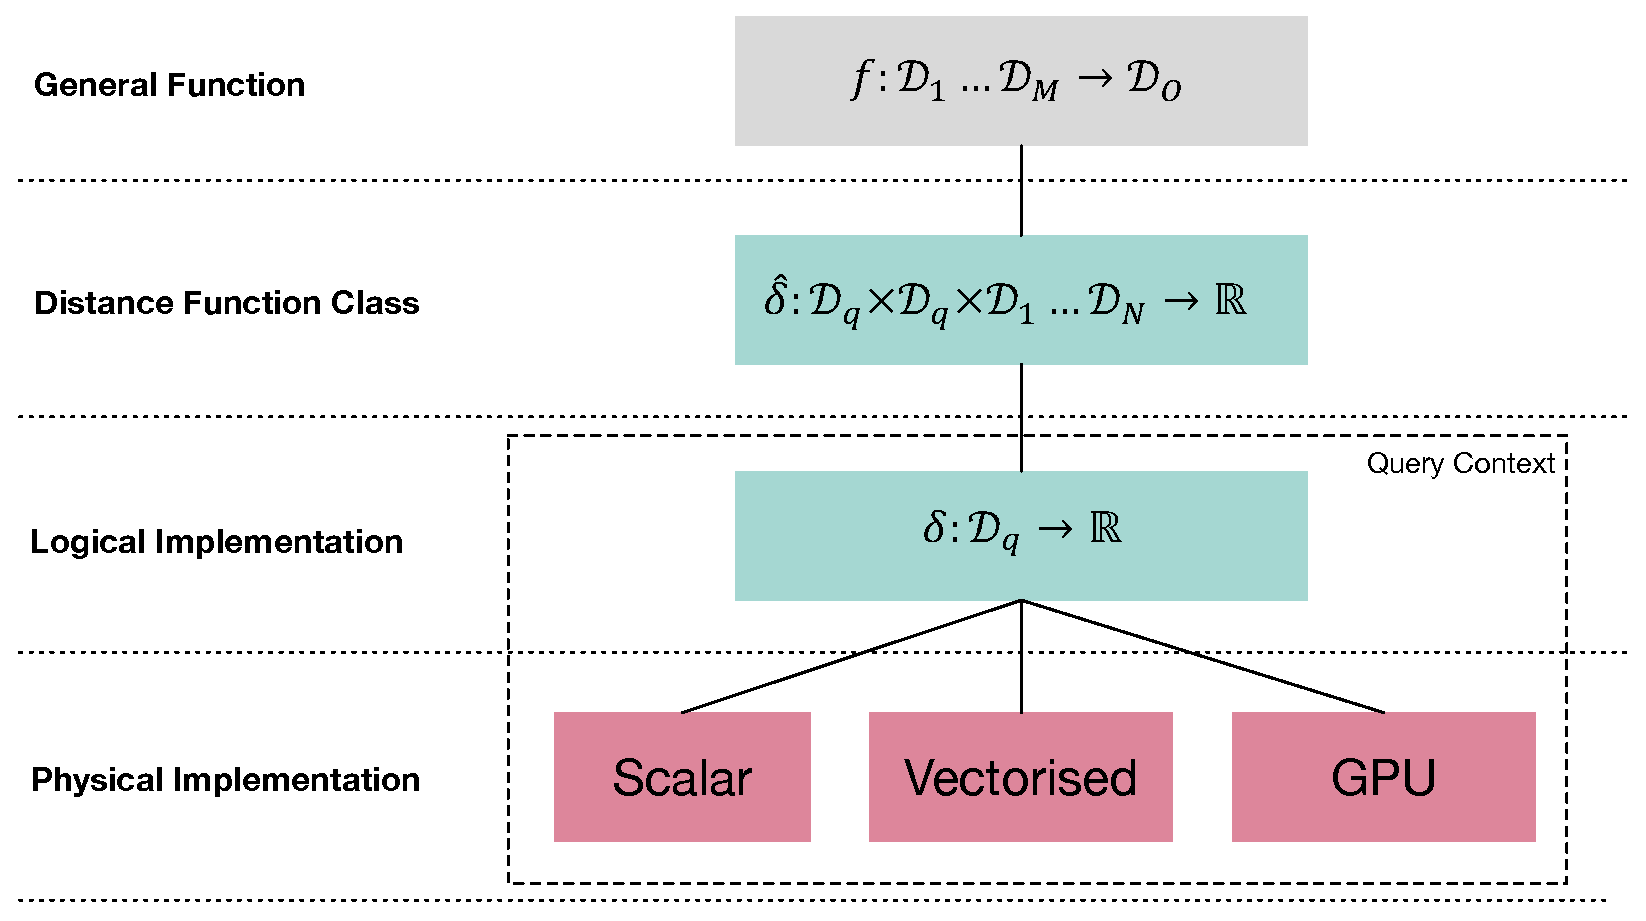
\includegraphics[width=\textwidth]{figures/function_hierarchy.eps}
    \caption{Function hierarchy of all $f \in \mathcal{F}$. As we go down the hierarchy, the \acrshort{dbms} gains knowledge about a function's structure.}
    \label{figure:function_hierarchy}
\end{figure}

\begin{description}
    \item[General Function] Every function $f \in \mathcal{F}$ is known with information about its name and domain (i.e., its signature $\mathtt{SIG}(f)$). This enables the \acrshort{dbms} to provide optimised implementations or replacements for composit operations.
    \item[Distance Function Class] Since DFCs constitute a specific type of function, we can embedd equivalences between a DFC and different types of index structures directly within the function registry. Those equivalences allow a query planner to select one over the other.
    \item[Logical Implementation] As an implementation of a query manifests, the structure of a DFC may change through implementation $\symdist = \mathtt{IMP}(\symdfc)$. For example, certain attributes may turn-out to remain constant, which can be leveraged by the planner to optimise execution.
    \item[Physical Implementation] As the physical execution plan emerges, a plan can make decisions as to what type of implementation for a DFC should be selected. For example, it may select a vectorised version, which leverages \acrshort{simd} instructions of the CPU, over a scalar implementation that calculates the distance in a tight loop.
\end{description}

Optimising implementations of DFCs and general function invocations can be achieved in multiple ways. First, it is reasonable to provide and select implementations that are specific for the data type of the function arguments, so as to avoid type conversion in a tight loop over a large amount of data. This is especially true for \acrshort{dfc}s that operate on complex datatypes, such as vectors. This goes into the direction of \Cref{requirement:complex_data_types}. 

Another aspect that can be optimised is the use of vectorised implementations for computations that involve vectors or matrices, i.e., exchanging a scalar implementation of a \acrshort{dfc} by an implementation that uses \acrshort{simd} instructions. This can be beneficial both for a multimedia \acrshort{dbms} that employs the iterator model and even more so for a batched processing model. However, for the iterator model it is to expected that one challenge lies in finding the threshold at which usage of such an optimised version pays off. If we take real-valued vectors as an example, it is likely that vectorised execution will not benefit low-dimensional vectors (e.g., $\text{dim} = 3$) while it will greatly benefit high-dimensional vectors (e.g., $\text{dim} = 2048$). Finding this threshold poses challenge in and by itself, which could be subject for future research.

Finally, one can try to match constellations of functions and replace them with an optimised version. A simple example could be the expression $a * b + c$, i.e., $\mathtt{add}(\mathtt{mul}(\mathtt{a},\mathtt{b}), \mathtt{c})$, which can be replaced by a single \emph{fused multiply-add} function $\mathtt{fma}(\mathtt{a},\mathtt{b},\mathtt{c})$ to avoid loss of precission. Replacing the evaluation of a \acrshort{dfc} with a lookup in a high-dimensional index also falls into this category, however, this transformation depends on more than just the function itself.

\subsection{\texorpdfstring{\acrshort{dfc}s}{DFCs} and High-Dimensional Index Structures}
\label{section:dfc_and_indexes}

One identity that is particularly relevant for the execution of proximity based queries is the relationship between the execution of a \acrshort{dfc} and the use of a high-dimensional index. As we have discussed in \Cref{section:hd_index_structures}, there exist many different types of indexing techniques that can be used to speed-up \acrshort{nns} in different ways. We propose to formalise the use of high-dimensional indexes\footnote{By ``index'' we refer to a concrete implementation rather than a family since all techniques introduced in \Cref{section:hd_index_structures} can be employed in different ways.} by definining equivalence classes between an index and the relational algebra expressions it replaces. For this, we rely on the index definitions presented in \Cref{section:databases_storage_manager}. In addition to \Cref{definition:index}, the following restrictions may apply in addition to implementation specific restrictions for a specific high-dimensional index: 
\begin{enumerate*}[label=(\roman*)]
    \item High-dimensional indexes are always derived from a feature attribute $\attribute_f \in \schema(\relation)$. Therefore, an index can only replace a DFC if they operate on an unaltered version of $\attribute_f$. Changes to $\attribute_f$, e.g., through application of a nested function $\mathtt{fun}(\attribute_f)$, will render the index unusable unless the same alteration was applied when creating the index.
    \item High-dimensional indexes are sometimes trained for a specific distance function (e.g., Euclidean) or class of distance functions (e.g., Minkowski). Therefore, an index can only replace an expression if the DFC used in that expression coincides with the original function (-class).
\end{enumerate*} Using these constraints, we can now formalise the replacement of a relational expression by an $\symindex^{\relation}_{I}$ which, for high-dimensional indexes and depending on what expression is matched, falls into one of three classes given by Definitions \ref{definition:dfc_index_class_1}, \ref{definition:dfc_index_class_2} or \ref{definition:dfc_index_class_3}.

\begin{definition}[label=definition:definition:index_replacement_exact]{Exact Index Replacement}{}
    Let $\relation$ be a relation, $\symplan$ a relational (sub-)expression (i.e., an execution plan) involving $\relation$ and $\symindex^{\relation}_{I}$ an index on $\relation$. We call the replacement of $\symplan$ with $\symindex^{\relation}_{I}$ an \emph{exact index replacement} if $\symplan \equiv \symindex^{\relation}_{I}$.
\end{definition}

\begin{definition}[label=definition:dfc_index_class_1]{High-Dimensional Index Replacement of Class 1}{}
    Let $\relation$ be a relation, $\attribute_f \in \schema (\relation)$ an attribute of $\relation$ , $\symdfc$ a \acrshort{dfc}, $q \in \domain_f$ a query and $\projection_{P}$ the extended projection involving execution of that \acrshort{dfc} using the query, i.e., $\symdist = \symdfc(\attribute_f, q, \ldots) \in P$. We call a replacement with a high-dimensional index $\symindex^{\relation}_{\attribute_f, \symdist} \equiv \projection_{\symdfc}(\relation)$ \emph{class 1}, if:

    \begin{equation*}
        \projection_{P} (\relation) = \projection_{\symdfc}(\relation) \Join_{\mathtt{TID}} \projection_{P \setminus \symdfc}(\relation) = \symindex^{\relation}_{\attribute_f, \symdfc} \Join_{\mathtt{TID}} \projection_{P \setminus \symdfc}(\relation)
    \end{equation*}
\end{definition}

Class 1 index replacements constitute the simplest and most versatile case. The index acts as a drop-in replacement for the distance calculation. One high-dimensional index-structures that can provide this functionality it the simplest variant of the \acrshort{pq} index, namely, the exhaustive SDC and ADC algorithms described in \cite{Jegou:2010Product} .

\begin{definition}[label=definition:dfc_index_class_2]{High-Dimensional Index Replacement of Class 2}{}
    Let $\relation$ be a relation, $\attribute_f \in \schema (\relation)$ an attribute of $\relation$ , $\symdfc$ a \acrshort{dfc}, $q \in \domain_f$ a query and $\projection_{P}$ the extended projection involving execution of that \acrshort{dfc} using the query, i.e., $\symdist =\symdfc(\attribute_f, q, \ldots) \in P$ and $\order_{\attribute_{d\updownarrow}}$ be an order operation involving the derived distance attribute $\attribute_{d}$. We call a replacement with a high-dimensional index  $\symindex^{\relation}_{\attribute_f, \symdfc} \equiv\order_{\attribute_{d\updownarrow}} (\projection_{\symdfc}(\relation)) $ \emph{class 2} if:

    \begin{equation*}
        \order_{\attribute_{d\updownarrow}}(\projection_{P} (\relation)) = \order_{\attribute_{d\updownarrow}}(\projection_{\symdfc}(\relation)) \Join_{\mathtt{TID}} \projection_{P \setminus \symdfc}(\relation) = \symindex^{\relation}_{\attribute_f, \symdfc} \Join_{\mathtt{TID}} \projection_{P \setminus \symdfc}(\relation)
    \end{equation*}
\end{definition}

Class 2 index replacements return a ranked relation that comes pre-sorted according to the derived distance in addition to obtaining the actual distance value.  This can be convenient for certain applications but it is also a rare trait and we do not have a concrete example of an index that provides this property. However, the caching of (sub-)queries could lead to such a replacement.

\begin{definition}[label=definition:dfc_index_class_3]{High-Dimensional Index Replacement of Class 3}{}
    Let $\relation$ be a relation, $\attribute_f \in \schema (\relation)$ an attribute of $\relation$ , $\symdfc$ a \acrshort{dfc}, $q \in \domain_f$ a query and $\projection_{P}$ the extended projection involving execution of that \acrshort{dfc} using the query, i.e., $\symdist =\symdfc(\attribute_f, q, \ldots) \in P$, $\order_{\attribute_{d\updownarrow}}$ an order operation involving the derived distance attribute $\attribute_{d}$, $\limit_k$ a $k$-selection and $\selection_{S}$ a selection involving a comparison of the distance attribute $\attribute_d$. We call a replacement with a high-dimensional index $\symindex^{\relation}_{\attribute_f, \symdfc} \equiv \texttt{OP}(\order_{\attribute_{d\updownarrow}} (\projection_{\symdist}(\relation)))$ with $\texttt{OP} \in \lbrace \limit_k, \selection_{S} \rbrace$ \emph{class 3} if:

    \begin{equation*}
        \texttt{OP}(\order_{\attribute_{d\updownarrow}}(\projection_{P} (\relation))) = \texttt{OP}(\order_{\attribute_{d\updownarrow}}(\projection_{\symdfc}(\relation))) \Join_{\mathtt{TID}} \projection_{P \setminus \symdfc}(\relation) =  \symindex^{\relation}_{\attribute_f, \symdfc} \Join_{\mathtt{TID}} \projection_{P \setminus \symdfc }(\relation)
    \end{equation*}
\end{definition}

Class 3 replacements constitute an optimisation of a specific edge-case, which is that of \acrshort{knn}, \acrshort{kfn} and or $\epsilon$NN search. It is probably the most common since it allows for most optimisation but is also the least versatile type of index replacement, since it merely supports one specific type of search. An example of such an index replacement is provided in \Cref{example:index_replacement}

\begin{example}[label=example:index_replacement]{Index Replacement for \acrshort{knn} Search}{}
    The following table lists the schema, extent and rank of $\relation^{\emptyset}_{\mathtt{painting}}$, with their title $\mathcal{A}_{\mathtt{(t)itle}}$, the year of their creation $\mathcal{A}_{\mathtt{(p)ainted}}$ and some arbitrary feature vector $\mathcal{A}_{\mathtt{(f)eature}}$. Let further $\symdfc$ be the Manhattan distance.

    \begin{center}
        \begin{tabular}{ l || l | l | l | l |}
            $\relation^{\emptyset}_{\mathtt{(p)ainting}}$ & $\attributep_{\mathtt{(t)itle}}$  & $\attributef_{\mathtt{(a)rtist}}$ & $\attribute_{\mathtt{(p)ainted}}$ & $\attribute_{\mathtt{(f)eature}}$ \\ 
            \hline
            \hline
            $t_1$ & Mona Lisa &  Leonardo da Vinci & 1506 &  $[2.0,7.0,-8.0]$ \\
            \hline
            $t_2$ & The Starry Night & Vincent van Gogh & 1889 & $[1.0.,0.0,3.0]$ \\
            \hline
            $t_3$ & Las Meninas & Diego Velázquez & 1665 & $[-1.0,3.0,9.0]$ \\
            \hline
            ... & ... & ... & ... & ... \\
            \hline
            $t_N$ & Mars and Venus & Sandro Botticelli & 1483 & $[-3.0,1.0,0.0]$ \\
            \hline
        \end{tabular}
    \end{center}

    The result of the \acrshort{knn}-search can be produced by a class 3 index replacement with $\symindex^{\relation_{p}}_{\attribute_f, \symdfc}$.
    
    \begin{equation*}
        \relation^{\mathcal{A}_d\uparrow}_{\mathtt{result}} = \lambda_k (\order_{\mathcal{A}_d\uparrow} ( \pi_{\mathcal{A}_{t}, \symdist(\mathcal{A}_{f})} ( \relation_p))) = \symindex^{\relation_{\mathtt{p}}}_{\attribute_f, \symdfc} \Join_{\mathtt{TID}} \projection_{\attribute_{t}} (\relation_p)
    \end{equation*}
    
    An index structure could be employed here is the \acrshort{vaf} index \cite{Weber:1998Va}.
\end{example}

With the aforementioned definitions and restrictions, we have defined the basic relationship and rules that can be applied by a multimedia \acrshort{dbms}, when deciding whether or not to use a high-dimensional index structure. However, the definitions so far consider the replacement an exact transformation, i.e., the result of the original expression and the index is supposed to be identical. In practice, this is often not the case, which leads to \Cref{definition:index_replacement_approximate}.

\begin{definition}[label=definition:index_replacement_approximate]{Approximate Index Replacement}{}
    Let $\relation$ be a relation, $\symplan$ a relational (sub-)expression involving $\relation$ and $\symindex^{\relation}_{I}$ an index on $\relation$. We call the replacement of $\symplan$ with $\symindex^{\relation}_{I}$ an \emph{approximate index replacement} if $\symplan \approx_{b} \symindex^{\relation}_{I}$ with:
    \begin{equation*}
        \symplan \approx_{b} \symindex^{\relation}_{I} \leftrightarrow Q(\symplan,\symindex^{\relation}_{I}) \geq b, b \in [0, 1]
    \end{equation*}

     $Q$ is a \emph{quality estimator} that derives a score between zero and one by comparing the results of $\symplan$ and $\symindex$.
\end{definition}  

In a manner of speaking, $\symplan$ acts a groundtruth and is compared to the approximate results produced by $\symindex^{\relation}_{I}$. The choice of quality metric $Q$ is implementation specific. One could, for example, pick recall if one is primarily interested in set-based overlap rather than the ranking of individual items, which is enough for unranked query plans:

\begin{equation*}
        Q_1(\symplan,\symindex) = \frac{|\symplan \cap \symindex|}{|\symplan|}
\end{equation*}

An alternative could be the use of a normalised \acrfull{dcg} \cite{Jarvelin:2002Cumulated}, if the ranking of items should be taken into account as well:

\begin{equation*}
    Q_2(\symplan,\symindex) = \frac{\mathtt{DCG}(\symplan,\symindex)}{\mathtt{iDCG}(\symplan)}
\end{equation*}

Regardless of the choice of metric, the challenge lies in predicting its value for a query prior to its execution. Since the result of $Q$ can only be produced in hindsight once a query has been executed, we need techniques to anticipate its value for an incoming query so that the \acrshort{dbms} can use this downstream to make decision about query execution.

\section{Cost Model for Multimedia Databases}
\label{section:cost_model}

As we have explained in \Cref{chapter:theory_databases}, most \acrshort{dbms} rely on a cost-model for planning and selecting the execution and access path of a user-specified query. In fact, ever since the System R paper \cite{Selinger:1979Access}, cost-based query planning and optimisation has been considered a gold standard for database systems \cite{Mannino:1988Statistical}. Most traditional \acrshort{dbms} exhibit cost-models that mainly rely on the cost incurred by accessing (reading / writing) database pages from or to disk \cite{Mannino:1988Statistical,Garcia:2009Database,Petrov:2019Database}. Based on what has been discussed thus far, we argue that this model must be adapted to be useful for multimedia databases so that it takes the following aspects into account when chosing a query execution plan:

\begin{description}
    \item[Disk Access (IO)] Persistent storage and the access to information residing on disk is the factor that contributes the most to long query execution times and is thus a factor to minimise \cite{Selinger:1979Access}. This is also true for proximity based queries, where part of the optimisation lies in reducing access to vectors through compression and/or early filtering, e.g., \cite{Weber:1998Va, Chierichetti:2007Finding}.
    \item[CPU] Due to the computational complexity of proximity based operations, especially when the evaluation of functions on high-dimensional vectors are involved, the processing time on CPU is a factor that can no longer be ignored and must thus be taken into account as well. In fact, several index structures achieve speed-up by reducing the computational complexity of the distance calculation \cite{Jegou:2010Product} or by avoiding it alltogether \cite{Weber:1998Va}.
    \item[Memory] Some algorithms can benefit greatly from pure in-memory processing. While memory used to be a scarce resource, some environments allow for complete in-memory processing even for very large datasets. This is exploited by systems like Milvus \cite{Wang:2021Milvus}, that load entire data collections into memory.
    \item[Quality] The quality of a result incurred, e.g., by the choice of a certain high-dimensional index structure \cite{Indyk1998:Approximate,Jegou:2010Product}, is a price that can be paid to attain speed-up. This is common practice in approximate \acrshort{nns} and should be made transparent to the system and user for reasons explained in \Cref{requirement:quality_model}, especially since this trade is not always viable (see \Cref{section:application_mrf}).
\end{description}

These four factors can be used to characterise query workloads in a purely local setup consisting of a single node. For distributed databases, the cost incurred by data and message exchange must obviously be considered as well. While this is not in scope for the work presented in this Thesis, the proposed model can be easily extended to accomodate those (and other) types of costs as well. The aforementioned factors lead us to \Cref{definition:op_cost} and \Cref{definition:plan_cost} for the cost incurred by an operator $\symop$ and query execution plan $\mathcal{P}$.

\begin{definition}[label=definition:op_cost]{Cost of a Relational Operator $\symop$}{}
    Let $\symop$ be a (relational) operator. We call the 4-tuple $C_{\symop} = (c_{\mathtt{IO}}, c_{\mathtt{CPU}}, c_{\mathtt{MEM}},c_{\mathtt{Q}})$ the \emph{cost} of $\symop$, which captures the atomic costs in terms of disk access (IO), CPU usage (CPU), memory usage (MEM) and quality (Q).
\end{definition}

\begin{definition}[label=definition:plan_cost]{Cost of a Query Exection Plan $\mathcal{P}$}{}
    Let $\symplan = \symop_1 \circ \symop_2, \ldots \circ \symop_N $ be a query execution plan consisting of $N$ operators. The plan's total cost $C_{\symplan}$ is given by the component-wise sum of the individual cost components:

    \begin{equation*}
        C_{\symplan} = \sum_{i=1}^{N} C_{\symop_i} = (\sum_{i=1}^{N} c_{\mathtt{IO},i}, \sum_{i=1}^{N} c_{\mathtt{CPU},i}, \sum_{i=1}^{N} c_{\mathtt{MEM},i}, \sum_{i=1}^{N} c_{\mathtt{Q},i})
    \end{equation*}
\end{definition}

\begin{example}[label=example:cost_model]{Cost of a Query Execution Plan}{}
    Let $\relation_{\mathtt{painting}}$ and $\relation_{\mathtt{artist}}$ be relations from \Cref{example:rel_alg_query}, the query ``return the names of all paintings that were painted by an artist who died after 1800'' results in the following, unoptimised execution plan:

    \begin{equation*}
        \symplan= \projection_{\attribute_{\mathtt{title}}}(\selection_{\attribute_{\mathtt{death}} > 1800}(\relation_{\mathtt{artist}} \Join \relation_{\mathtt{painting}}))
    \end{equation*}

    This query gives rise to following operator tree with individual and total costs (the cost factors are purely illustrational and do not relate to any real values):

    \begin{center}
        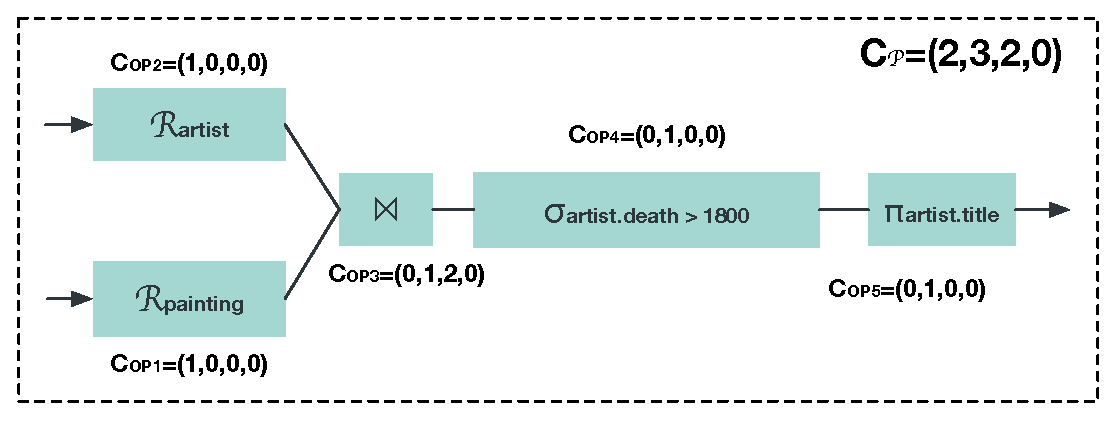
\includegraphics[width=0.90\textwidth]{figures/cost_example.eps}
    \end{center}
\end{example}

The role of $C_{\symplan}$ is twofold: First, its absolute values can be used by the \acrshort{dbms} to determine hard constraints imposed for query execution. For example, if there is a fixed limit on memory that can be used by a query, an execution plan may be discarded simply based on exceeding that memory limit regardless of other factors. Similarily, a hard constraint on quality could be imposed. Second, it can be used to compare execution plans relatively to one another. \Cref{example:cost_model} illustrates cost calculation for a simple execution plan.

The cost factors per operator can be determined in many ways and the model does not assume any specific approach with the exception for $c_{\mathtt{Q}}$, which will be described in \Cref{section:quality_cost_estimation}. However, we do require that the method for determining the factors must be internally consistent and should not change so as to keep costs comparable. For illustrative purposes, we outline the following, rough metrics to estimate $c_{\mathtt{IO}}$, $c_{\mathtt{CPU}}$, $c_{\mathtt{MEM}}$: IO cost can be estimated by the number of bytes that must be read / written by an operator. This is equivalent to the estimated number of tuples read $T$ times the estimated size of a tuple in bytes (atomic IO cost $a_{\texttt{IO}}$ in bytes). One can also introduce a correction factor $c$ to distinguish between different types of access (e.g., sequential random).

\begin{equation*}
    c_{\mathtt{IO}} = a_{\texttt{IO}}Tc
\end{equation*}

CPU cost can be estimated by the number memory accesses and/or the number of arithmetic operations and or memory accesses that are executed by an operator (atomic CPU cost $a_{\texttt{CPU}}$ in operations) times the number of tuples $T$ being processed.

\begin{equation*}
    c_{\mathtt{CPU}} = a_{\texttt{CPU}}T
\end{equation*}

Memory cost can be estimated by the size of the in-memory data structures maintained by an operator (e.g., for sorting or hash-joins), i.e., the number of tuples materialised in memory $T_m$ times the size of a tuple (atomic memory cost $a_{\texttt{MEM}}$ in bytes)

\begin{equation*}
    c_{\mathtt{MEM}} = a_{\texttt{MEM}}T_m
\end{equation*}

Since the atomic costs stem from completely different domains and are therefore not directly comparable and because we only compare plans relative to one another, we require a cost normalisation step, which we base on available plan candidates $\mathcal{P}_1$ and which is outlined in \Cref{definition:cost_normalisation}.

\begin{definition}[label=definition:cost_normalisation]{Cost Normalisation}{}
    Let $\mathtt{PLANS} = \mathcal{P}_1, \ldots, \mathcal{P}_N$ be $N$ equivalent query execution plans with associated costs $\mathtt{COSTS} =C_{\mathcal{P}_1}, \ldots,C_{\mathcal{P}_N}$. We consider the maximum cost $C_{\mathtt{max}}$ for those plans to be the component-wise maximum of all $C_{\mathcal{P}} \in \mathtt{COSTS}$. Using $C_{\mathtt{max}}$, the normalised cost $ C_{\mathcal{P},i,\mathtt{norm}}$ can be expressed as:

    \begin{equation*}
        C_{\mathcal{P},i,\mathtt{norm}} = (\frac{c_{\mathtt{IO},i}}{c_{\mathtt{IO},\mathtt{max}}},\frac{c_{\mathtt{CPU},i}}{c_{\mathtt{CPU},\mathtt{max}}},\frac{c_{\mathtt{MEM},i}}{c_{\mathtt{MEM},\mathtt{max}}},\frac{c_{\mathtt{Q},i}}{c_{\mathtt{Q},\mathtt{max}}})
    \end{equation*}

    It follows from the definition, that each component of a normalised cost falls into an interval between $0$ and $1$ due to the normalisation, i.e., $c_{\mathtt{*},\mathtt{norm}} \in [ 0, 1 ]$.
\end{definition}

It is important to note, that the normalised cost can only be used for relative comparison within an existing set of plans. It generally does not provide any information about the original cost value and the underlying properties they may represent. Using this normalised costs, we can now derive \emph{cost score} according to \Cref{definition:cost_score}.

\begin{definition}[label=definition:cost_score]{Simple Cost Score}{}
    Let $\mathcal{P}$  be a query execution plan with associated, normalised cost $C_{\mathcal{P}_{\mathtt{norm}}}$. We consider the \emph{cost score} to be the sum of the atomic costs.

    \begin{equation*}
        \mathcal{S} = c_{\mathtt{IO},\mathtt{norm}} + c_{\mathtt{CPU},\mathtt{norm}} + c_{\mathtt{MEM},\mathtt{norm}} + c_{\mathtt{Q},\mathtt{norm}}
    \end{equation*}

    The basic cost score $ \mathcal{S}$ falls into an interval between $0$ and $N$ wherein $N$ denotes the number of atomic costs, i.e., $\mathcal{S} \in [0, $N] for $N = |C_{\mathcal{P}_{\mathtt{norm}}}|$.
\end{definition}

The cost score $\mathcal{S}$ can be used to directly compare query plans in a given context and, e.g., sort them in ascending order during plan enumeration in order to select the one plan that minimises the costs. However, it assumes that all the components have the same importance, which in practice is often not the case.

\subsection{Cost Policies}

The definitions employed so far treat every component of a cost $C_{\mathcal{P}_{\mathtt{norm}}}$ equally with regards to the resulting cost score $\mathcal{S}$. This is rarely desirable since the different components influence the outcome to a different extent (e.g., in terms of query execution time or result quality). This can be expressed by employing a \emph{cost policy} as outlined in \Cref{definition:cost_policy}.

\begin{definition}[label=definition:cost_policy]{Cost Policy and Weighted Score}{}

    Let $\mathcal{P}$  be a query execution plan with associated, normalised cost $C_{\mathcal{P}_{\mathtt{norm}}}$. We call the 4-tuple $\mathcal{W}$ a cost-policy.

    \begin{equation*}
        \mathcal{W} = (w_{\mathtt{IO}}, w_{\mathtt{CPU}}, w_{\mathtt{MEM}}, w_{\mathtt{Q}}), \text{ with } w_{\mathtt{IO}},  w_{\mathtt{CPU}}, w_{\mathtt{MEM}}, w_{\mathtt{Q}} \in [0, 1]
    \end{equation*}

   The weighted cost score $\mathcal{S}_{\mathcal{W}}$ with respect to $\mathcal{W}$ can be expressed as the linear combination of $C_{\mathcal{P}_{\mathtt{norm}}}$ and $\mathcal{W}$:

    \begin{equation*}
        \mathcal{S}_{\mathcal{W}} = C_{\mathcal{P}_{\mathtt{norm}}} \cdot \mathcal{W} = w_{\mathtt{IO}}c_{\mathtt{IO},\mathtt{norm}} + w_{\mathtt{CPU}} c_{\mathtt{CPU},\mathtt{norm}} + w_{\mathtt{MEM}} c_{\mathtt{MEM},\mathtt{norm}} + w_{\mathtt{Q}} c_{\mathtt{Q},\mathtt{norm}}
    \end{equation*}
\end{definition}

The cost policy provides us with a blunt but simple instrument to assign importance to individual cost factors. For example, one can prioritise execution speed by assigning more weight to the CPU and IO components or one can favour the quality of the results by having a high $w_{\mathtt{Q}}$. In an actual multimedia \acrshort{dbms} implementation, $\mathcal{W}$ can be influenced at different levels, which supersede one another, namely 
\begin{enumerate*}[label=(\roman*), itemjoin={{, }}, itemjoin*={{, or }}, after={{.}}]
    \item as a system-wide configuration
    \item for a user-session (connection-level) or transaction
    \item for an individual query
\end{enumerate*} 
Consequently, different users should have the ability to express different preferences in terms of cost policy.

\subsection{Estimating Cost of Approximation}
\label{section:quality_cost_estimation}

In order to complete the cost model, we must generate an estimate of how the quality of a result is influenced by chosing a particular execution plan over another. While the described model is kept general, it is directly related to the approximate index replacement problem given in \Cref{definition:index_replacement_approximate}. We propose a simple method that involves a post-hoc evaluation of results to estimate the quality measure at different levels using the quality function $Q$.

\begin{definition}[label=definition:cost_estimation_quality]{Cost Estimate based on Quality Estimation}{}
    Let $\symplan_1$, $\symplan_2$ be two equivalent query plans and $\limit_k$ the $s,k$-selection. Let further $Q$ be a quality estimator that derives a score by comparing the results produced by $\symplan_1$ and $\symplan_2$. The cost estimate for quality $c_{Q,k}$ at a given level $k$ is then is given as:
    
    \begin{equation*}
        c_{Q,k,\symplan} = 1 - q_k = 1 - Q(\limit_k(\symplan_1),\limit_k(\symplan_2))
    \end{equation*}
\end{definition}

For proximity based queries, $\symplan_1$, $\symplan_2$ are two equivalent query plans that do and don't involve the evaluation of an approximate, high-dimensional index. In practice, the obtained numbers for $c_{Q,k}$ can be stored in a lookup-table and updated on a regular basis (e.g., when querying the index anyway). In case no observation is available, one can provide a \emph{cost prior}, which is an index-dependent estimate of the cost. Furthermore, the \acrshort{dbms} can alsoo pre-calculate certain costs factors on the known classes of high-dimensional index replacements described \Cref{section:dfc_and_planning} and likely queries. Whenever a query is being planned, the \acrshort{dbms} can lookup the estimates.

As indicated by the indexes $k$ and $\symplan$, we estimate $c_{Q,k,\symplan}$ at multiple levels $k$ and for different families of plans. We propose a logarithmic progression of the ranking levels, e.g., $k= \{ 1, 2, 4, 8, \ldots \}$ for two reasons: Firstly, the probability of an extreme value is higher for lower than for higher levels. This is also visualised in \Cref{figure:index_quality}. Secondly, items with a lower rank are often considered more relevant than items exhibiting a high rank \cite{Jarvelin:2002Cumulated}, i.e., we require a more accurate estimate for lower levels.

While the model is very simple it obviously only provides a rough estimate. Furthermore, there are some important implicit assumptions we operate upon: Firstly, we assume that the quality of an execution plan depends on the type of plan and not on the query parameters provided by the user (e.g., the vectors used for proximity based search). The underlying assumption is, that the query parameters are being drawn from the same, (albeit unknown) probability distribution that has produced the indexed data. We believe this to be a reasonable assumption, because as we have argued in \Cref{chapter:theory_multimedia_analysis_and_retrieval}, these vectors are usually produced by some well-defined feature transformation. To illustrate this, we plot the average recall and normalised \acrshort{dcg} for the results produced by a \acrshort{pq}-based index implementation over a $1000$ different queries in \Cref{figure:index_quality}. \footnote{Based on the Yandex Deep 1B dataset \cite{Babenko:2016Efficient} and the provided groundtruth query vectors.} We can observe that the mean remains more or less constant over different levels approaching $1.0$ as the level is being increased. However, the minimum and maximum show a much larger spread for lower levels which is a purely stochastical phenomenon. The second assumption is, that the quality of the results at lower, constrained ranking levels provides a valid estimator for quality at higher levels, i.e., that the agreement is continued indefinitely. Both assumptions require some ``well-behavedness'' of the index structure and concrete configurations thereof, which may not necessarily be a given.

\begin{figure}
    \centering
    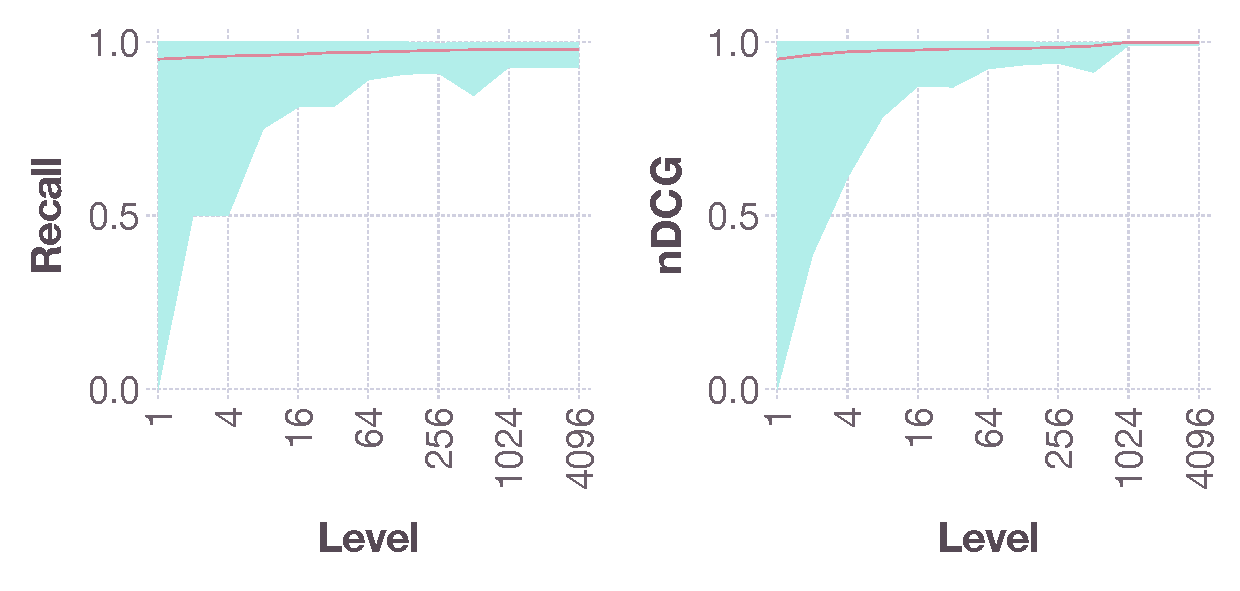
\includegraphics[width=\textwidth]{figures/index-quality-pq}
    \caption{Quality of results produced by a \acrshort{pq} index in a \acrshort{nns} query in terms of recall and normalised \acrshort{dcg} at different levels observed and averaged over a $1000$ queries using different query vectors. The mean value remains more or less constant while minimum and maximum exhibit a large spread for smaller levels.}
    \label{figure:index_quality}
\end{figure}

\section{High-Dimensional Index Maintenance}
\label{section:hd_index_maintenance}

Maintining a consistent and predictable behaviour of (high-dimensional) index structures is imperative for a multimedia \acrshort{dbms} to guarantee a constant quality of service level or even \acrshort{acid} properties, for that matter. While the challenge of maintaining durable index structures and handling incremental as well as concurrent updates to them is a well studied problem (e.g., for the $B^{+}$-tree index \cite{Garcia:2009Database,Petrov:2019Database}), the on-disk storage and maintenance of high-dimensional indexes is not \cite{Amsaleg:2014Database}, with the exception of a few, isolated examples \cite{Olafsson:2011Dynamic,Hojsgaard:2019Index,Jayaram:2019DiskANN,Lu:2020VHP}. In addition to practical considerations, e.g., how data structures designed for use in main memory can be optimised for disk access to guarantee durability, there is the fundamental problem of an index's ability to cope with changes to the data in a consistent manner, especially when concurrent read and write access is involved. What makes the issue challenging is that, as we have demonstrated in \Cref{section:hd_index_structures}, many different types of algorithms exist for high-dimensional indexing, all of which bring their own characteristics. Since the problem of dynamic, high-dimensional indexing on secondary storage has not been widely considered in literature and is in fact often ignored by the inventors of new indexing methods, \footnote{It is either assumed that data is static or that re-indexing the entire collection is an option.} there are no established best practices as to how to handle the issue \cite{Olafsson:2011Dynamic,Amsaleg:2014Database}.

In this section, we propose a model to accomodate and maintain different types of durable high-dimensional index structures in a consistent manner. The model is supposed to be applicable to any tpye of index and considers it to be an auxiliary data structure, that provides certain (potentially imperfect) operations that enable us to make incremental changes to it. Furthermore, indexes in this model exhibit an explicit state that allows the \acrshort{dbms} to make decisions as to if and how the index can be used. Failure of an index due to accumulating changes is an explicit scenario that must be handled by the system. The proposed model consists of a series of components, based on which it can operate. Those are:
\begin{enumerate*}[label=(\roman*)]
    \item A \emph{storage model},
    \item a \emph{write model} and,
    \item a \emph{failure- and associated cost model} for every type of index,
    \item a system-wide notion of transaction isolation and
    \item the ability to (re-)build an index from scratch.
\end{enumerate*} 
The model can be applied for any type of index and we will see, that a ``traditional'' index structure can be considered a specific corner-case of the model.

\subsection{Storage Model}

The basic assumption and prerequisite is that all the high-dimensional index structures offered by the \acrshort{dbms} always act as secondary indexes. Consequently, the primary data (i.e., the original vectors) are always stored without loss of information and in a manner that allows for seamless propagation of changes, e.g., as index- or heap-organised tables in the case of a relational database. \footnote{This is an approach (implicitly) taken by methods such as DiskANN \cite{Jayaram:2019DiskANN}, however, for the simple reason that in-memory storage is not feasable for large collections.} At this point, we re-iterate the formal definition of a secondary index $\symindex^{\relation}_I$ with respect to the relation $\relation$ it indexes from \Cref{definition:index} and the related \Cref{equation:index_attribute_reconstruction} that enables us to reconstruct attributes that are missing in the index using the primary data.

The fallback strategy that the \acrshort{dbms} therefore can always resort to, in case an index becomes unavailable, is that of a sequential scan of the original data, which results in a higher latency for reasons discussed in \Cref{section:multimedia_retrieval}, and should therefore be avoided. Furthermore, the primary data files can be used to reconstruct the index. Since, to the best of our knowledge, all publications on high-dimensional indexes outline the steps required to rebuild index from a data collection, we can safely assume that this is always possible. Moreover, the primary data can be used to correct missing or outdated information on the fly at query time, e.g., using random lookups.

In addition to this basic requirement, one must consider how the in-memory representation of a particular index can be efficiently mapped to disk. Refering to the list of indexes presented in \Cref{table:index_structures}, a naive mapping is often straightforward. Many indexes are organised as lists, maps or trees and can therefore be organised using the persistent version of the respective data structure. At a high level, if an index is always scanned in its entirety, an array or list may be the easiest and most efficient form of storage. One could, for example, use a binary association table-like structure as used by MonetDB \cite{Idreos:2012MonetDB} to map \texttt{TID} to signature. If an index can benefit from filtering, e.g., to restrict a scan to a subset of the index in an inverted file \cite{Chierichetti:2007Finding,Gudmundsson:2010Large,Jegou:2010Product}, then a ($B^{+}$-)tree structure might be more beneficial, which brings the advantage that we know how to maintain it. In practice, there are many caveats to sort out, such as, balancing the size of clusters in clustered indexes \cite{Hojsgaard:2019Index} and distributing data in a way that minimises unnecessary page access \todo{1-2 additional sources}. We consider these to be important but index-specific aspects, which are not the focus of this chapter.

\subsection{Write Model of an Index}
An index's write model characterises its ability to incorporate changes into the data structures outlined by its storage model. To lay the groundwork, we formalise the notion of a change to a relation in the form of three operations listed in \Cref{definition:change}. 

\begin{definition}[label=definition:change]{Change Operations to Relation $\relation$}{}
    Let $\relation$ be a relation and $t \in \relation$, $t^{\prime} \in \relation^{\prime}$ tuples with $\schema(\relation) = \schema(\relation^{\prime})$. We call $\symchangeop(\relation,\cdot) \in [ \mathtt{INSERT}(\relation, \cdot), \mathtt{DELETE}(\relation, \cdot), \mathtt{UPDATE}(\relation, \cdot) ]$ a change operation on $\relation$ and the quadruple $\symchange = (\symchangeop, \relation, t, t^{\prime})$ a \emph{change}.

    \begin{align*}
        \mathtt{INSERT}(\relation, t^{\prime}) &= \relation \cup \lbrace t^{\prime} \rbrace \\
        \mathtt{DELETE}(\relation, t ) &= \relation \setminus \lbrace t \rbrace \\
        \mathtt{UPDATE}(\relation, t, t^{\prime}) &= ((\relation \setminus \lbrace t \rbrace) \cup \lbrace t^{\prime} \rbrace)\\
    \end{align*}

    That is, $\symchangeop(\relation,\cdot)$ can be used to add, remove or replace tuples in $\relation$. These operations correspond to the basic \acrshort{crud} operations available to a \acrshort{dbms}. It is worth noting that formally, we can decompose any \texttt{UPDATE} operation into a consequtive \texttt{INSERT} and \texttt{DELETE}.
\end{definition}

The write model $\symwritem_{\symindex}$ is now a function as given by \Cref{definition:write_mode}. It decides for every change $\symchange$ if and how it can be propagated to index $\symindex$ and applies it, if possible. In case a change $\symchange$ can be applied successfully, the write model returns \texttt{true}. If the change cannot be propagated, the write model returns \texttt{false}. In both cases, the change is forwarded to the index's failure model alongside the outcome $W$ of the write model.

\begin{definition}[label=definition:write_mode]{Write Model for Index $\symindex$}{}
    Let $\relation$ be a relation and $\symindex$ an index on attributes $I \subset \schema(\relation)$. The write model $\symwritem_{\symindex}$ is a function that determines, if a change $\symchange = (\symchangeop, \relation, t, t^{\prime})$ can be applied to the index given additional parameters $P = \{p_1, p_2, \ldots p_n\}$:

    \begin{equation*}
        \symwritem_{\symindex}(\symchange,P) = 
        \begin{cases}
           \mathtt{true}, & \text{if } \symchangeop(\relation,t,t^{\prime}) \text{ can be applied to } \symindex \\
           \mathtt{false}, & \text{otherwise}
        \end{cases}
    \end{equation*}
\end{definition}

The application of $\symwritem_{\symindex}$ always takes place within the context of the transaction $\symtrans_c$ that has issued the change and it therefore inherits all guarantees provided by it. Most importantly, all (side-)effects of $\symwritem_{\symindex}$ are only made visible to other transactions upon \texttt{COMMIT} and are completely negated by a \texttt{ROLLBACK}.

\subsection{Failure Model and State of an Index}

The failure model $\symfailm_{\symindex}$ is a second function as given by \Cref{definition:failure_model} that determines the new state of the index given change $\symchange$, the result of the write model $W$ and optional parameters $P = \{p_1, p_2, \ldots p_n\}$ (e.g., up-to-date index statistics).

\begin{definition}[label=definition:failure_model]{Failure Model for Index $\symindex$}{}
    Let $\relation$ be a relation and $\symindex$ an index on attributes $I \subset \schema(\relation)$. The failure model $\symfailm_{\symindex}$ is a function that determines the index's new state $S \in \lbrace \mathtt{CLEAN}, \mathtt{DIRTY}, \mathtt{STALE} \rbrace$ given a change $\symchange = (\symchangeop, \relation, t, t^{\prime})$, the outcome of the write model $W$ and parameters $P = \{p_1, p_2, \ldots p_n\}$:

    \begin{equation*}
        \symfailm_{\symindex}(\symchange,W,P) = 
        \begin{cases}
           \mathtt{CLEAN}, & \text{if change can be applied without imparing the index}\\
           \mathtt{DIRTY}, & \text{if change may impair the index}\\
           \mathtt{STALE}, & \text{if change leads to index failure} \\
        \end{cases}
    \end{equation*}
\end{definition}

Based on the outcome of the failure model, the index's state and cost characteristics can be updated. The state determines, if and how the index can be used for query execution and thereby enforces consistent results within the quality parameters provided by the \acrshort{dbms}. The cost characteristic allows for more fine grained control, in case, certain cost factors are directly influenced by a change (or an accumulation thereof), for example, if changes lead to a deterioration in quality. We distiguish between three states as illustrated in \Cref{figure:failure_model}:

\begin{description}
    \item[Clean] indexes are ready for use by the \acrshort{dbms} and able to produce results within the speed and quality parameters they naturally provide.
    \item[Dirty] indexes are ready for use by the \acrshort{dbms}. However, the flag signals that an index's ability to produce results within speed and quality parameters is impaired. This flag is usually accompanied by adjustments to the cost characteristic of the index that account for this.
    \item[Stale] indexes have stopped functioning within their defined parameters and are therefore removed from consideration for query planning. Reason for this state is often an inconsistency, e.g., due to a missing record.
\end{description}

Freshly (re-)built indexes start in the \texttt{CLEAN} state. If the write model fails for a change $\symchange$, i.e., $\symwritem(\symchange,P) = \mathtt{false}$, the state is updated to \texttt{STALE} and the index becomes unavailable and is marked for rebuilding. However, even if the write model succeeds, the change may still trigger a transition to either the \texttt{DIRTY} or the \texttt{STALE} state, if the changes that have accumulated in the meanwhile are expected to lead to index deterioration that goes beyond a certain threshold. Internal statistics can be consulted and updated to, e.g., adjust the index's cost model.

Again, we require that the application of $\symwritem_{\symindex}$ -- including all updates to state and cost model -- take place within the context of the transaction $\symtrans_c$ that has issued the change. Consequently, it also inherits all guarantees and is subject to its \texttt{COMMIT} and \texttt{ROLLBACK} semantics.

\begin{figure}[bt]
    \centering
    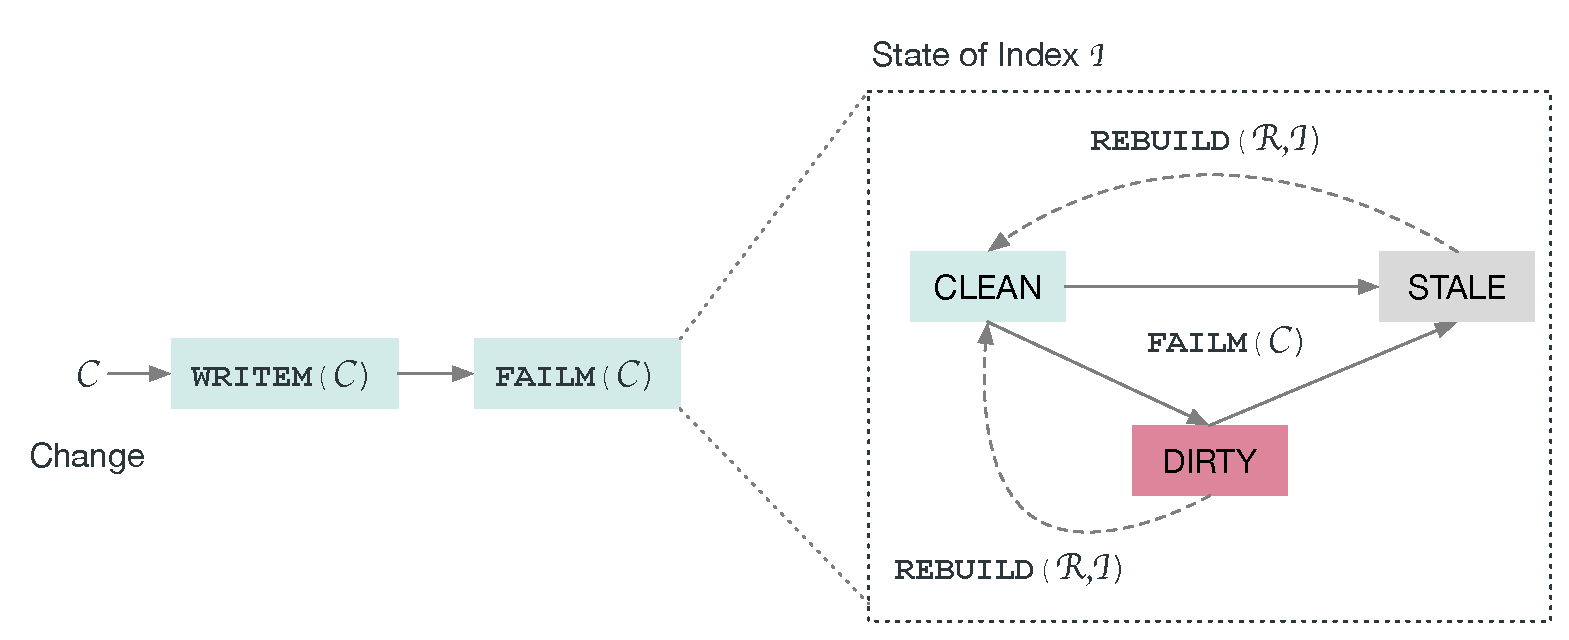
\includegraphics[width=\textwidth]{figures/failure_model.eps}
    \caption{Illustration of a change $\symchange$ to the data that is process by an index $\symindex$'s write- and failure model and leads to potential state changes. An index knows the three states \texttt{CLEAN}, \texttt{DIRTY} and \texttt{STALE}.}
    \label{figure:failure_model}
\end{figure}

\subsection{Concurrent Index Rebuilding}

Once an index has been marked as \texttt{STALE} it can no longer be used by the \acrshort{dbms} until it is rebuilt by the $\symrebuild(\relation,\symindex,P)$ function, where $P = \{ p_, p_2, \ldots p_n \}$ again denotes a list of additional parameters. In essence, the rebuild function simply re-constructs the index $\symindex$ based on the primary data held in $\relation$.

Using this model, we prevent a faulty index from generating potentially erroneous results, e.g., if entries go missing because they could not be added. Hence, we can ensure consistency even as potentially unprocessable changes accumulate. However, the failure of an index means that the \acrshort{dbms} must resort to a sequential scan, which may negatively impact query performance. This can only be remediated by an index rebuild, which is often a long-running process that may take several minutes to hours for large datasets to complete. A time during which, new changes may arrive.

This is why we propose an algorithm that minimises conflicts with other, concurrent database operations. As a pre-requisite for this algorithm to work, we assume that every transaction $\symtrans_t$ operates on a consistent snapshot $\symsnap_t$ of the database state at the time $t$ when the transaction started. This is a concurrency control mechanism known as \emph{snapshot isolation} \cite{Berenson:1995Critique}, which is very common in modern \acrshort{dbms}. In this section, we will refer to snapshots of relations and indexes with subscripts, e.g.,  $\relation_{1} \in \symsnap_1$ is a relation and $\symindex_{1} \in \symsnap_1$ is an index for $t=1$. The rebuilding of a (high-dimensional) index can now be separated in two steps: The \texttt{BUILD} and the \texttt{REPLACE} phase, which start at timepoints $s$ and $r$ respectively, with $s < r$. The basic assumption behind separating these two steps is, that building up the index structure is the time consuming part, while merging the index to the persistent data structures (i.e., writing it to disk) is faster, since it does not involve any access to the primary data nor any complex computations. Hence, the aim of our approach is to minimise exclusive access to the primary data structures maintained by the \acrshort{dbms}. The entire algorithm is also illustrated in \Cref{figure:async_index_rebuild}.

During the \texttt{BUILD} phase, the primary data in $\relation_{s}$ is scanned in a read-only transaction $\symtrans_{s}$ and the obtained data is used to build up the data structures required by the index. The constructed data structure exists outside of a proper database snapshot and is therefore not part of any visible database state other than $\symtrans_{s}$ \footnote{We do not make any assumptions as to whether the structure is built in-memory or on disk.}. We therefore refer to this as a \emph{shadow index} $\symindex^{\prime}$. Since transaction $\symtrans_{s}$ is read-only, concurrent reads and writes to the database can take place and all transaction $\symtrans_{s \geq t < r}$ will see the state of the original $\symindex_{s < t < r}$ at the given point in time, regardless of whether that index is still operational (\texttt{CLEAN}), in process of deterioration (\texttt{DIRTY}) or has failed in the meanwhile (\texttt{STALE}). 

The index build-up is followed by the \texttt{REPLACE} phase, which takes place in a second transaction $\symtrans_{r}$ that follows directly after $\symtrans_{s}$ and writes the shadow index created during the \texttt{BUILD} to the \acrshort{dbms} snapshot $\symsnap_r$ and then commits that snapshot. $\symtrans_{r}$ is a write transaction and may require exclusive access on the data structures involved. It replaces the $\symindex_{r-1}$ with an updated version $\symindex_{r}$ that can take over. All transactions $\symtrans_{t \geq r}$ will see the state of the newly built index $\symindex_{t \geq m}$. 

Separating these two steps obviously ignores one important aspect, which is that of change operations that take place between timepoints $s$ and $r$. Since the \texttt{SCAN} phase operates on snapshot $\relation_{s}$, those are not taken into account when rebuilding the index. We solve this, by introducing an additional \emph{side-channel} between $\symtrans_{s}$ and concurrent transactions $\symtrans_{s < t < m}$ that \texttt{LEAK} relevant information. Every concurrent transaction that commits successfully, reports all relevant changes to the entity that orchestrates the \texttt{REBUILD} operation, which will be responsible for merging these changes with the shadow index $\symindex^{\prime}$ using its write- and failure model. In practice, this can be realised as some kind of event-bus allowing for a \emph{publish-subscribe} like communication model. The entity that orchestrates the rebuild can then subscribe to changes of the relation it is scanning.

\subsubsection{Failure Cases and Limitations}

The proposed algorithm has several failure cases that must be handled and limitations that must be addressed. Obviously, $\symrebuild(\relation,\symindex,P)$ fails, if the leaking process fails (i.e., information is lost) or if during the \texttt{BUILD} phase, the shadow index becomes unusable, i.e., its failure model signals a problem with some of the leaked information. In both cases, the shadow index must be discarded and rebuilding of the index must be and resumed from scratch in a new, up-to-date transaction. Therefore, for this algorithm to work, the index's write model should bring a certain degree of robustness to accumulating changes . 

Since the likelihood of accumulating enough changes for the rebuild to fail increases with runtime, the algorithm can also be combined with other strategies to reduce time spent in the critical \texttt{BUILD} phase, e.g., by having multiple, smaller partitions of the primary data in $\relation$ being (re-)built independently. \footnote{Such a model can also make sense if we consider partitioning of data during parallel execution and/or distribution.} This is a strategy, e.g., employed by Milvus \cite{Wang:2021Milvus} and formally, this leads to an index $\symindex$ that is composed of multiple sub-indexes, each with a shared write- and failure model but their own state. The state of the index is then determined by the state of its sub-indexes .

Last but not least, it is important to note that the proposed solution becomes a poweful tool if index failure can be (approximately) anticipated. Presuming this is possible, the index rebuild can be started ahead of time while the original index $\symindex$ is still functional. Due to snapshot isolation, concurrent read transactions can continue to use the original index until the new version becomes available. In addition to heuristics (e.g, after $x$ change operations the index is being rebuilt) one can also leverage the cost model proposed in \Cref{section:cost_model} to determine if index quality is deteriorating.

\begin{figure}
    \centering
    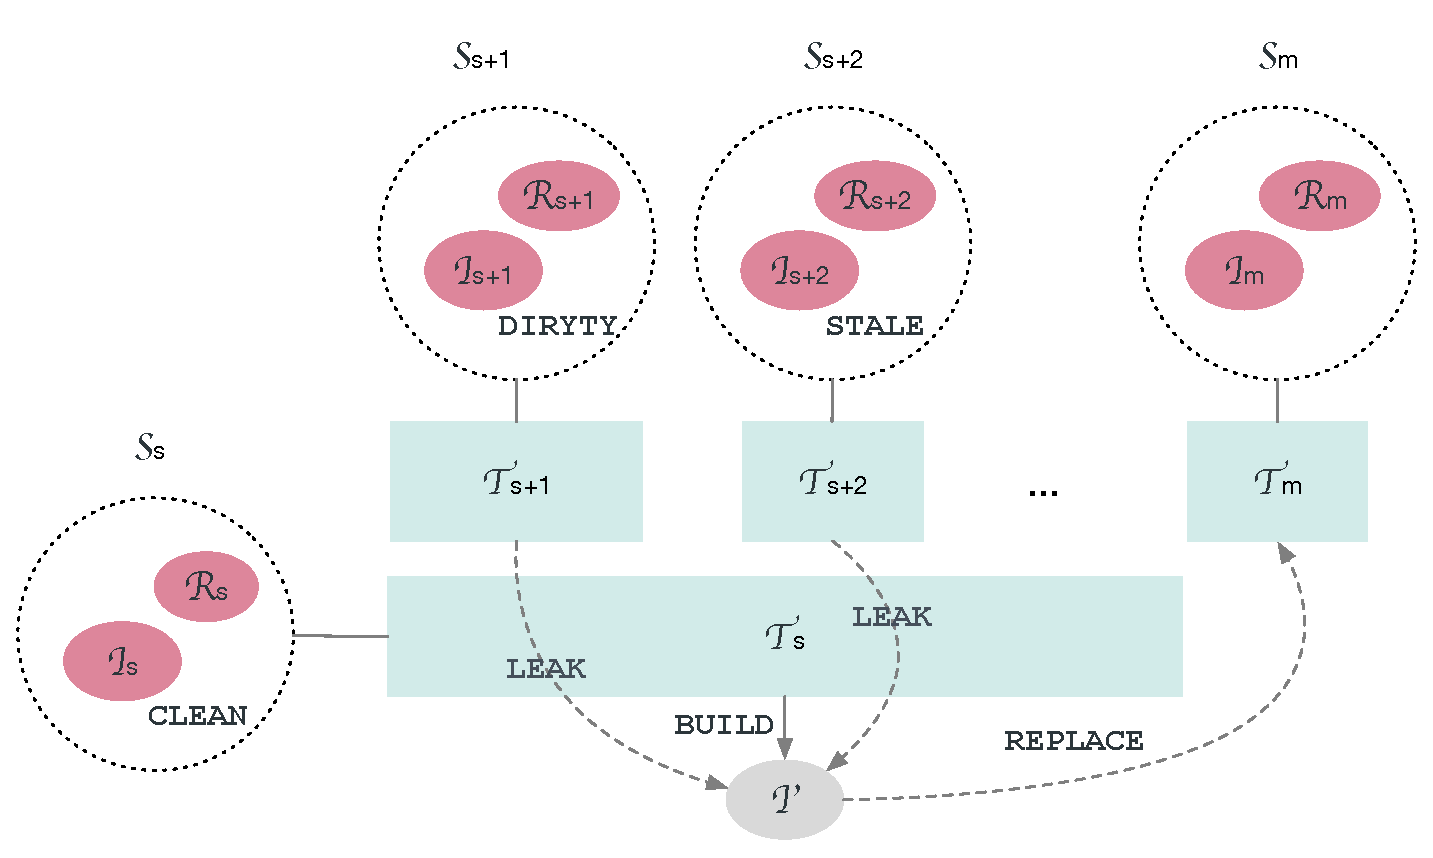
\includegraphics[width=\textwidth]{figures/asynchronous-index-rebuilding}
    \caption{Illustration of the asynchronous index rebuilding process, which takes place in two separate phases \texttt{BUILD} and \texttt{SCAN}. Information from transactions that take place concurrently to the  \texttt{BUILD} process are \texttt{LEAK}ed through a side-channel upon commit of the respective transaction.}
    \label{figure:async_index_rebuild}
\end{figure}

\subsection{Case Studies}

We illustrate the idea of the write- and failure model using two index structures \acrshort{vaf} \cite{Weber:1998Va} and \acrshort{pq} \cite{Jegou:2010Product}. These case studies serve as mere examples and the concepts themselves can be applied to other indexes as well.

\subsubsection{Write and Failure Model for \texorpdfstring{\acrfull{vaf}}{VAF}}

The \acrshort{vaf} (see \Cref{section:index_vaf}) algorithm assigns a vector $f$ to a cell in a high-dimensional lattice that is determined by a partitioning the vector space. That partitioning is derived from the component-wise minimum and maximum $f_{l}$ and $f_{u}$ of all feature vectors $f \in \domain_f$. From that we can determine the write model for a relation $\relation$ with the attribute $\attribute_f$ of data domain $\domain_f \subset \symreal^d$ with $d \in \symnatural_{>0}$. The \texttt{INSERT} is illustrated in \Cref{equation:write_model_insert_vaf} and \Cref{figure:write_model_insert_vaf}.

\begin{equation}
    \label{equation:write_model_insert_vaf}
    \symwritem_{\mathtt{VAF}}((\mathtt{INSERT}, \relation, t^{\prime}),f_{l},f_{u}) =
    \begin{cases}
        \mathtt{true} & \text{if } f_{l,i} \geq t^{\prime}[\attribute_f]_i \geq f_{u,i} \forall i \in [1,d]\\
        \mathtt{false} & \text{otherwise}
    \end{cases}
\end{equation}

When a new tuple $t^{\prime}$ is inserted, the write model for the \acrshort{vaf} index must check if the vector $t^{\prime}[\attribute_f]$ falls into bounds of the component-wise minimum and maximum vector. If it does, then the signature can be calculated directly and appended to the list -- the write model returns $\mathtt{true}$. Otherwise, the vector's position in the grid is undefined and the write model should return $\mathtt{false}$. However, to harden the index for those types of failures, one can introduce the notion of a \emph{tombstone marker}, \footnote{The idea is inspired by Apache Cassandra, which uses tombstones to mark deleted entries. See, for example, \cite{Padalia:2015Apache}.}, which indicates an entry that is out of bounds for the current index configuration. This could, for example, be a pre-defined number ($-1$ in the illustration shown in \Cref{figure:write_model_insert_vaf}). Instead of writing the signature, the write model would then simply write the marker. When the index is scanned and a marker is encountered, the vector for that entry is fetched from the primary data and the exact distance is calculated. This leads to a deterioration of query speed, since more vectors must be read from disk.

\begin{figure}
    \centering
    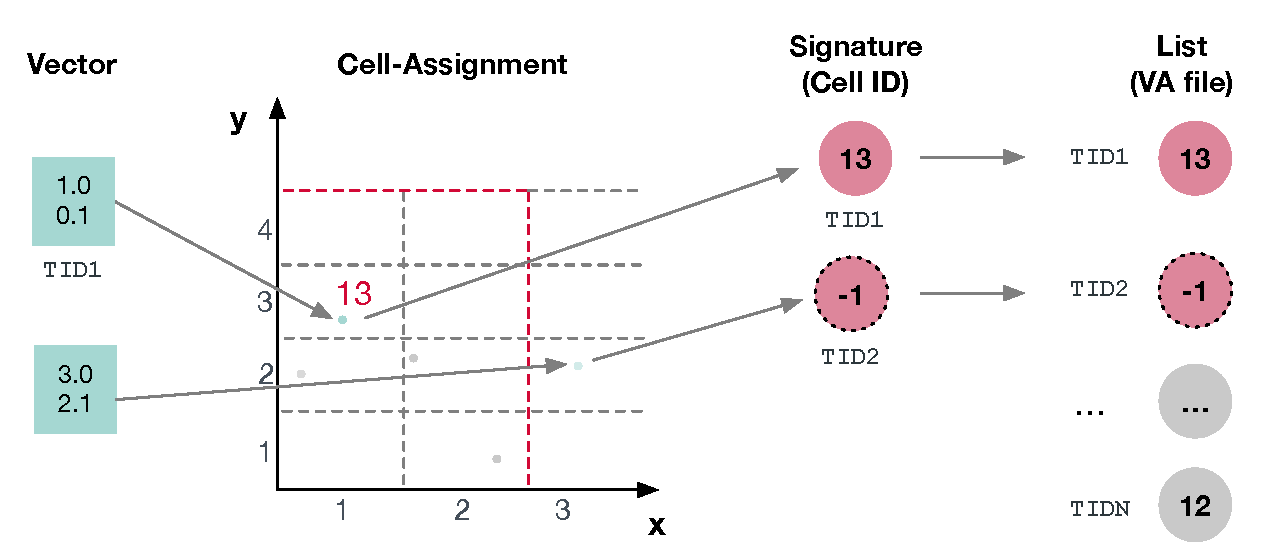
\includegraphics[width=\textwidth]{figures/vaf-write-model}
    \caption{Illustration of the \acrshort{vaf} index's write model (insert). If a vector lies within the bounds spanned by the minimum and maximum, the signature can be appended. If not, a tombstone marker can be generated and appended to the VA-file instead.}
    \label{figure:write_model_insert_vaf}
\end{figure}

If an existing tuple $t \in \relation$ is removed, then this change can be applied in any case. The signature is simply looked-up and removed from the list. However, as deletes accumulate, the component-wise minimum and maximum of the $\domain_f$ may shift, which potentially leads to an overly large and therefore sparsely populated lattice.

\begin{equation}
    \label{equation:write_model_delete_vaf}
    \symwritem_{\mathtt{VAF}}(\mathtt{DELETE}, \relation, t) = \mathtt{true}
\end{equation}

Formally, the ability to apply an update can be directly expressed as a combination of $ \symwritem_((\mathtt{INSERT}, \relation, t^{\prime}),\cdot)$ and $ \symwritem((\mathtt{DELETE}, \relation, t), \cdot)$, as outlined in \Cref{definition:change}. In practice, the two steps would be merged into a dedicated operation to optimise performance.

The failure model must now determine, how to handle the aforementioned changes. Both the sparsenes of the overlay grid as well as the accumulation of tombstone markers will potentially lead to a deterioration of the index's ability to produce results in a reasonable amount of time. Hence, as these changes accumulate, the need for an index rebuild becomes more pressing. As a very simple option, the \acrshort{dbms} could determine a fixed threshold after which an index will go \texttt{STALE} or after which re-indexing will be triggered. While simple to realise, it is probably difficult to find a good estimate for the threshold.

Alternatively, one can use the \acrshort{vaf} index's filtering capability as a measure. According to \cite{Weber:1998Va}, a typical VA-file should be able filter-out between 90 and 99\% of the candidates without accessing the original vectors. That number can be used as a default value. Every time an index is scanned, when executing a query, that value can be updated (for free) and with it, the index's cost model. Eventually, the index will be removed from consideration automatically as the cost of scanning it exceeds the cost of a full table scan. 

\subsubsection{Write and Failure Model for \texorpdfstring{\acrfull{pq}}{PQ}}
\acrshort{pq} (see  \Cref{section:index_pq}) involves quantisation of a vector based on the assignment to a list of centroids in a codebook. The resulting signature is then either stored in list (\acrshort{pq}) or an inverted index (IVF\acrshort{pq}). For both \acrshort{pq} and IVF\acrshort{pq}, the quantiser used to construct the original index can be stored and re-used to process changes to the data. Consequently, an incoming vector is simply quantised and appended to the respective data structure and the write model for a (IVF-)\acrshort{pq} should always return \texttt{true}, as indicated by \Cref{equation:write_model_insert_pq}.

\begin{equation}
    \label{equation:write_model_insert_pq}
    \symwritem_{\mathtt{PQ}}(\mathtt{INSERT}, \relation, t^{\prime}) = \mathtt{true}
\end{equation}

Similarily, for deletes, the entry associated with the deleted \texttt{TID} can be removed from the list. One can arrange \texttt{TID} and associated signature in a tree structure to accelerate this lookup. In the case of an IVF\acrshort{pq} index, the procedure incurs some additional overhead, since for a successful delete, the original vector must be read and its position in the inverted index must be determined by applying the coarse quantiser. Subsequently, that slot must be scanned until the entry with the deleted \texttt{TID} can be found. In any case, the write model should return true as indicated by \Cref{equation:write_model_insert_pq}.

\begin{equation}
    \label{equation:write_model_delete_pq}
    \symwritem_{\mathtt{PQ}}(\mathtt{DELETE}, \relation, t) = \mathtt{true}
\end{equation}

Again, formally, the ability to apply an update can be directly expressed as a combination of $\symwritem(\mathtt{INSERT}, \relation, t^{\prime})$ and $ \symwritem(\mathtt{DELETE}, \relation, t)$, as outlined in \Cref{definition:change}. In practice, the two steps would probably be merged into a dedicated operation, to optimise performance.

The failure model of a \acrshort{pq} must potentially take multiple aspects into account. Firstly, a quantiser learned for a given size of the collection may become non-representative of the collection as it grows, especially if the growth exceeds orders of magnitude (e.g., from $100000$ to $1000000$ entries). Secondly, a growing number of potentially very similar vectors may lead to a degeneration of the indexes ability to distinguish between vectors. And lastly, for IVF\acrshort{pq}, the different clusters constructed by coarse quantisation may become imbalanced over time. In all these cases, complete re-indexing with potentially different parameters may be required\footnote{It is to be noted, that finding the optimal choice of parameters given a collection is still a poorly understood problem \cite{Ge:2014Optimized}.}.